% !TEX root = epifanov_solid_state_physics.tex
%!TEX TS-program = pdflatex
%!TEX encoding = UTF-8 Unicode


\chapter[Electrical Conductivity of Solids]{Electrical Conductivity of Solids}\label{chap:6}
% \chaptermark{The Band Theory of Solids}

\section{Equilibrium state of electron gas in a conductor in the absence of an electric field}\label{sec:47}

In the absence of an electric field, the electron gas in a conductor is in an equilibrium state described by equilibrium distribution functions. For a degenerate gas the appropriate function is the Fermi-Dirac distribution function [\fig{6_1}(a)] and for a nondegenerate gas the Maxwell-Boltzmann distribution function [\fig{6_1}(b)].

It may be seen from \fig{6_1} that the graphs of those functions are symmetric about the axis of ordinates. This points to the fact that the number of electrons in a conductor moving in the opposite directions is always the same and their average velocity in any direction is zero. This explains the fact that there is no electric current in a conductor (in the absence of a field), no matter how many free electrons it contains.

The equilibrium of the electron gas is established as a result of the interaction of the electrons with the lattice defects, this interaction being accompanied by energy and momentum exchanges. Such defects include thermal vibrations of the lattice (phonons), lattice imperfections, and impurity atoms. The interaction results in electron scattering and their random motion in the conductor.

\begin{figure}[t]
	\begin{center}
		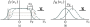
\includegraphics[scale=1]{figures/ch_06/fig_6_1.pdf}
		\caption[]{The Fermi-Dirac (a) and Maxwell-Boltzmann (b) distribution functions.}
		\label{fig:6_1}
	\end{center}
	\vspace{-0.7cm}
\end{figure}

\section{Electron drift in an electric field}\label{sec:48}

When an electric field $\vec{\mathcal{E}}$ is applied to a conductor, an electric current is established in it whose density according to Ohm's law is
\begin{equation}\label{eq:6_1}
    \vec{i} = \sigma \vec{\mathcal{E}}.
\end{equation}

\noindent
The proportionality factor a is termed the \textit{specific conductance} of the conductor. Its dimensions are \si{\per\ohm\per\centi\metre} or \si{\per\ohm\per\metre}. Good conductors have $\sigma\approx$ \SIrange{e7}{e8}{\per\ohm\per\metre}; good dielectrics \SIrange{e-12}{e-14}{\per\ohm\per\metre}. Often, it is more convenient to use the \textit{specific resistance}
\begin{equation}\label{eq:6_2}
    \rho = \frac{1}{\sigma}
\end{equation}

\noindent
instead of specific conductance.

The specific resistance is measured in \si{\ohm\metre}. For metals $\rho\approx$ \SIrange{e-7}{e-8}{\ohm\metre}; for dielectrics $\rho\approx$ \SIrange{e12}{e14}{\ohm\metre}.

A current flowing in the conductor is an indication of the fact that electrons acted upon by the field begin to move in a specific direction and that their distribution function experiences a change. Such directional motion is termed \textit{drift} and the average velocity of this
motion---\textit{drift velocity} $\ab{\vec{v}}{d}$. Let us calculate it.

The force with which the field $\vec{\mathcal{E}}$ acts on an electron is $\vec{F}=-q\vec{\mathcal{E}}$ (\fig{6_2}). Acted upon by this field the electron should be accelerated and its velocity should grow continuously. But in its motion the electron collides with the lattice defects and as a result of scattering
looses the velocity it gained in the field. The effect of the lattice may be formally reduced to the action of a resistance force $\ab{\vec{F}}{r}$, which hinders the electron in its motion through the lattice. This force is proportional to $\ab{\vec{v}}{d}$ and is directed against it:
\begin{equation}\label{eq:6_3}
    \ab{\vec{F}}{r} = - \frac{1}{\tau} \ab{m}{n} \ab{\vec{v}}{d}
\end{equation}

\noindent
with $1/\tau$ a proportionality factor whose physical meaning will be made clear subsequently, and $\ab{m}{n}$ the electron's effective mass.

\begin{figure}[t]
	\begin{center}
		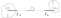
\includegraphics[scale=1]{figures/ch_06/fig_6_2.pdf}
		\caption[]{Forces acting on a free electron in a conductor in which an electric field $\mathcal{E}$ has been established.}
		\label{fig:6_2}
	\end{center}
	\vspace{-0.7cm}
\end{figure}

Using \eqn{6_3}, we may write the equation of the directional motion of the electron in the lattice in the following form:
\begin{equation}\label{eq:6_3p}
    \ab{m}{n} \diff{\ab{\vec{v}}{d}(t)}{t} = -q\vec{\mathcal{E}} - \frac{1}{\tau} \ab{m}{n} \ab{\vec{v}}{d}(t). \tag{6.3$'$}
\end{equation}

We see from \eqn{6_3p} that, after the field had been applied, the velocity of the directional motion of the electrons shall rise and the electrons shall be accelerated until the resistance force $\ab{\vec{F}}{r}$, which is proportional to $\ab{\vec{v}}{d}(t)$, shall become equal to the force $\vec{F}$ with which the field acts on the electron. When those forces become equal, the resultant force acting on the electron and, accordingly, its acceleration, shall vanish.

From this moment the directional motion of the electron shall proceed at a constant velocity
\begin{equation}\label{eq:6_4}
    \ab{\vec{v}}{d} = - \frac{q \vec{\mathcal{E}} \tau}{\ab{m}{n}}.
\end{equation}

\noindent
Since the electron charge is negative, its drift is in the direction opposite to $\vec{\mathcal{E}}$.

The ratio of the drift velocity to the field intensity is termed carrier mobility:
\begin{equation}\label{eq:6_5}
    u = \frac{\ab{v}{d}}{\mathcal{E}} = \frac{q\tau}{\ab{m}{n}}.
\end{equation}

\noindent
For electrons $\ab{u}{n}<0$, and for holes $\ab{u}{p}>0$.

According to \eqn{6_4}, the drift velocity in a field of constant intensity remains constant. This is possible only if the force $\vec{F}=-q\vec{\mathcal{E}}$ with which the field acts on the electron is compensated by the force $\ab{\vec{F}}{r}$. Would the opposite be the case the drift velocity would grow continuously and could become infinitely high even in weak fields. In this case, the electrical conductance would be infinite and the electrical resistance would vanish.

This would be the case if free electrons moved in an ideal regular lattice with a strictly periodic potential. The electron wave that describes the behaviour of the electron in such a lattice would propagate in it practically without attenuation, similar to a light wave propagating in an optically transparent medium.

The causes of a finite electrical resistance are various lattice imperfections, which result in the deformation of the lattice periodic potential and which serve as scattering centres for the electron waves, and attenuate the directional flux of the electrons in the same way as light waves are scattered and a ray of light is attenuated in an opaque medium.

\section{Relaxation time and mean free path}\label{sec:49}

Let us now find the physical meaning of the factor $\tau$.

Suppose that as soon as the velocity of the directional motion of the electrons attains its stationary value $\ab{v}{d}$, the field $\mathcal{E}$ is turned off. Because of the collisions of the electrons with the lattice defects this velocity will start to diminish and the electron gas will return to the state of equilibrium. Such processes leading to the establishment
of equilibrium in a system that was previously put out of it are termed \textit{relaxation processes}.

Setting $q\mathcal{E}=0$ in \eqn{6_3p} yields an equation describing the return of the electron gas to the equilibrium state, that is, the relaxation process
\begin{equation}\label{eq:6_6}
    \diff{\ab{v}{d}(t)}{t} = - \frac{1}{\tau} \ab{v}{d}(t).
\end{equation}

\noindent
Integrating \eqref{eq:6_6}, we obtain
\begin{equation}\label{eq:6_7}
    \ab{v}{d}(t) = \ab{v}{d}\, e^{-t/\tau}
\end{equation}

\noindent
where $\ab{v}{d}(t)$ is the velocity of the directional motion of the electrons, ($t$ is the time after the field had been turned off).

It follows from \eqn{6_7} that, $\tau$, \textit{characterizes the rate at which the equilibrium state of the system is established}: the less $\tau$ is, the sooner the excited system will return to the state of equilibrium. The velocity of directional motion of the electrons during the time $t=\tau$ decreases $e\approx 2.7$ times. The time $\tau$ is termed \textit{relaxation time}. For pure metals $\tau\approx\SI{e-14}{\second}$.

The motion of the electrons in a crystal may conveniently be described with the aid of the concept of mean free path. By analogy with the kinetic theory of gases, one may presume that an electron in a crystal moves along a straight line until it meets a lattice defect and is scattered. The average distance, $\lambda$, that the electron travels between two consecutive scattering acts is taken as the \textit{mean free path} of the electron.

Should the electron loose its directional velocity completely already after a single scattering act returning to the former state of random motion, its mean free path would simply be the product of its average velocity and the relaxation time $\tau$, which in this case would simply be the free transit time of the electron:
\begin{equation}\label{eq:6_8}
    \lambda = v \tau.
\end{equation}

However, often it is not one but on the average $\nu$ collisions with scattering centres that are required to nullify the directional velocity completely. Only after $\nu$ collisions, do all traces of correlation between the initial and the final velocities of the electron disappear. The time during which the directional motion of the electron becomes randomized will, in this case, too be termed relaxation time. However, the mean path the electron travels during this time is no longer $\lambda$, but
\begin{equation}\label{eq:6_9}
    l = \nu \lambda = v \tau.
\end{equation}

\noindent
The quantity $l$ is termed \textit{transport mean free path}.

It follows from \eqn{6_9} that
\begin{equation}\label{eq:6_10}
    \tau = \frac{\nu \lambda}{v}.
\end{equation}

\noindent
The appearance of the drift of free charge carriers resulting in an electric current is an indication of the fact that, the field $\mathcal{E}$ changes the distribution of free electrons over the states, that is, the form of the distribution function $f(E)$, since the equilibrium distribution function $f_0(E)$ cannot be the cause of the current. The dotted lines in Figures \ref{fig:6_1}(a,b) show the graphs of the electron distribution functions after a constant drift velocity had been established. It may be seen from \fig{6_1} that the effect of the field $\mathcal{E}$ on the electron distribution function over the states, is to shift the whole distribution by an amount $\ab{v}{d}=q\mathcal{E}\tau/\ab{m}{n}$ in the direction opposite to $\mathcal{E}$. Because of that shift, the distribution functions are no longer symmetric about the axis of ordinates and the average velocity of the
electrons in the direction of the $x$ axis is no longer zero (in the absence of the field this velocity was zero). It may be easily demonstrated that the average velocity will, in this case, be equal to the drift velocity $\ab{v}{d}$.

\section{Specific conductance of a conductor}\label{sec:50}

Knowing the drift velocity of the electrons $\ab{v}{d}$, we can easily calculate the current density and the specific conductance of a conductor. To this end, imagine a cylinder with a unit base built inside a conductor with a side equal to $\ab{v}{d}$ and directed along the direction of drift (\fig{6_3}). All the electrons inside this cylinder will in one second pass through the base establishing a current with a density
\begin{equation}\label{eq:6_11}
    \vec{i} = -q n \ab{\vec{v}}{d} = qnu \mathcal{E}.
\end{equation}

\begin{figure}[t]
	\begin{center}
		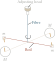
\includegraphics[scale=1]{figures/ch_06/fig_6_3.pdf}
		\caption[]{Calculating current density in a conductor.}
		\label{fig:6_3}
	\end{center}
	\vspace{-0.7cm}
\end{figure}

\noindent
Comparing \eqn{6_11} with \eqref{eq:6_1}, we obtain
\begin{equation}\label{eq:6_12}
    \sigma = qnu.
\end{equation}

\noindent
Substituting $u$ from \eqn{6_5} and $\tau$ from \eqn{6_10}, we obtain
\begin{equation}\label{eq:6_13}
    \sigma = \frac{n q^2}{\ab{m}{n}} \tau = \frac{n q^2}{\ab{m}{n}} \frac{\nu \lambda}{v}.
\end{equation}

\section{Electrical conductivity of nondegenerate
and degenerate gases}\label{sec:51}

Up to now, we did not distinguish between the nondegenerate and degenerate electron gases. Let us now try and find how the state of an electron gas affects its electrical conductivity. To this end, we shall discuss in more detail the conductivity mechanism of the nondegenerate and the degenerate gases in more detail.

\textbf{Nongenerate gas.} In the case of a nondegenerate gas, the occupancy of the conduction band by electrons is so small that they practically never come so close together that their behaviour is limited by the Pauli exclusion principle. The electrons are perfectly free in the sense that the motion of any one of them is not noticeably affected by the others. Therefore, all the conduction electrons of a nondegenerate gas play an independent part in the electric current and in the electrical conductivity of the conductor. For this reason, formulae \eqref{eq:6_5}
and \eqref{eq:6_13} for the electrical conductivity of the nondegenerate gas and for the electron mobility should include the mean free path $\overline{\lambda}$, the average number of collisions $\overline{\nu}$, the average velocity of motion $\overline{v}$, and the average relaxation time $\overline{\tau}$ of all the free electrons obtained by averaging over the ensemble as a whole.

Taking this into account, we can write the expressions for the electron mobility and for the specific conductance of a nondegenerate gas in the following form:
\begin{align}
    u &= \frac{q \overline{\tau}}{\ab{m}{n}} = \frac{q}{\ab{m}{n}} \frac{\overline{\lambda} \overline{\nu}}{\overline{v}},\tag{6.5$'$}\label{eq:6_5p}\\
    \sigma &= \frac{n q^2}{\ab{m}{n}} \overline{\tau} = \frac{n q^2}{\ab{m}{n}} \frac{\overline{\lambda} \overline{\nu}}{\overline{v}}.\tag{6.13$'$}\label{eq:6_13p}
\end{align}

\textbf{Degenerate gas.} The case of a degenerate gas is different. It may be seen from \fig{6_1}(a) that for a degenerate gas, all quantum states to the left of $\ab{v}{F}$ are occupied by electrons. Because of that, the external field can act only on the electrons close to the Fermi level, lifting them to higher vacant levels by moving them from the left-hand region of the distribution to the right-hand region, as shown by the arrow $11'$. This means that in a degenerate gas, only the electrons in the immediate vicinity of the Fermi level can take part in electrical conductivity. Therefore, one should take for the relaxation time in expressions \eqref{eq:6_5} and \eqref{eq:6_13}, the relaxation time of the electrons whose energy is practically equal to the Fermi energy. Let us denote it by $\ab{\tau}{F}$.

Substituting $\ab{\tau}{F}$ for $\tau$ in \eqref{eq:6_5} and \eqref{eq:6_13}, we obtain the following expressions for the electron mobility and the specific conductance of a degenerate gas:
\begin{align}
    u &= \frac{q\ab{\tau}{F}}{\ab{m}{n}} = \frac{q\ab{\lambda}{F} \ab{\nu}{F}}{\ab{v}{F}},\tag{6.5$''$}\label{eq:6_5pp}\\
    \sigma &= \frac{n q^2}{\ab{m}{n}} \ab{\tau}{F} = \frac{n q^2}{\ab{m}{n}} \frac{q\ab{\lambda}{F} \ab{\nu}{F}}{\ab{v}{F}}.\tag{6.13$''$}\label{eq:6_13pp}
\end{align}

\noindent
where $\ab{\lambda}{F}$ is the mean free path of the electrons with Fermi energy, $\ab{v}{F}$ their velocity, and $\ab{\nu}{F}$ the number of collisions after which the directional velocity of such electrons becomes randomized.

Here is, a rough mechanical analogy to explain the different behaviour of a nondegenerate and a degenerate electron gas in an electric held.

Imagine small charged balls (``particles'') floating on the surface of water in a flat horizontal vessel A and moving at random with different velocities in the absence of an external field [\fig{6_4}(a)]. Now, let us place this vessel in an external field $\vec{\mathcal{E}}$. The resulting effect of the field on the ensemble of the balls, as a whole, will substantially depend on how closely the balls are packed on the surface of water. If the number of balls is small, so that the distances between them are large, every one of them will move freely, practically speaking, and will not interfere with the motion of its neighbours [\fig{6_4}(a)]. In this instance the motion of the ensemble, as a whole, shall be determined by the average parameters of motion of the individual ``particles'': by the average velocity $\overline{v}$, by the average elaxation time $\overline{\tau}$, by the mean free path $\overline{\lambda}$, etc.

\begin{figure}[t]
	\begin{center}
		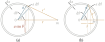
\includegraphics[scale=1]{figures/ch_06/fig_6_4.pdf}
		\caption[]{Mechanical model of the behaviour in of (a) a nondegenerate and (b) a degenerate electron gas; arrows denote the drift velocity in the electric held.}
		\label{fig:6_4}
	\end{center}
	\vspace{-0.7cm}
\end{figure}

If the balls are packed as closely as possible, so that there is no place for any more balls on the water's surface, then the motion of the ensemble as a whole under the action of the field $\vec{\mathcal{E}}$ will be determined by the motion of the lower layer of the ``particles'', CC, which separates the ``occupied'' states from the ``vacant'' states [\fig{6_4}(b)], namely, by the velocity of those particles $\ab{v}{C}$, by the relaxation time $\ab{t}{C}$, by the mean free path $\ab{\lambda}{C}$, etc. In a degenerate electron gas, the part of this layer is played by electrons close to the Fermi level, which separates occupied states from the vacant ones.

\section{Wiedemann-Franz-Lorenz law}\label{sec:52}

The transport of electric charge in an electric field is not the only result of the presence of the electron gas in a solid---another is heat transport in the presence of a temperature gradient. For this reason, it would be natural to expect that the electric and the heat conductivities of a solid are interrelated. This interrelation was first experimentally established by G. Wiedemann and P. Franz and theoretically explained by L. Lorenz for the case of metals. They showed the ratio of the heat conductivity $\mathcal{K}$ of a metal to its specific conductance a to be proportional to the absolute temperature $T$:
\begin{equation}\label{eq:6_14}
    \frac{\mathcal{K}}{\sigma} = LT.
\end{equation}

Expression \eqref{eq:6_14} is the essence of the \textit{Wiedemann-Franz-Lorenz law}; the proportionality factor $L$ is called the \textit{Lorenz number}.

The Wiedemann-Franz-Lorenz law can easily be obtained if one makes use of the expressions for $\mathcal{K}$ and $\sigma$ derived in the electron theory of metals. Dividing \eqn{4_58} for the heat conductivity of a metal (which is practically equal to its electron component) by \eqn{6_13pp}, we obtain
\begin{equation}\label{eq:6_15}
    \frac{\mathcal{K}}{\sigma} = \frac{\pi^2}{3} \parenthesis{\frac{\ab{k}{B}}{q}}^2 T.
\end{equation}

\noindent
Comparing \eqn{6_15} with \eqn{6_14}, we find that theoretical value of the Lorenz number
\begin{equation}\label{eq:6_16}
    L = \frac{\pi^2}{3} \parenthesis{\frac{\ab{k}{B}}{q}}^2 = \SI{2.45e-8}{\watt\ohm\per\kelvin\squared}.
\end{equation}

Table \ref{fig:6_1} shows the experimental values of $L$ for some pure metals at \SI{0}{\degreeCelsius}. We see that the theoretical value of $L$ agrees well with experiment.

\begin{table}[!b]
	\renewcommand{\arraystretch}{1.2}
	\caption{}
	\vspace{-0.6cm}
	\label{table:6_1}
	\begin{center}\resizebox{0.8\linewidth}{!}{
			\begin{tabular}{lccccccc}
				\toprule[1pt]
                & Ag & Au & Cd & Cu & Ir & Mo & Pb\\
                \midrule[0.5pt]\midrule[0.5pt]
                $L$ (\SI{e8}{\watt\ohm\per\kelvin\squared}) & $2.31$ & $2.35$ & $2.42$ & $2.23$ & $2.49$ & $2.61$ & $2.47$\\
				\bottomrule[1pt]
			\end{tabular}
	}\end{center}
\end{table}

In semiconductors with a nondegenerate electron gas the heat conductivity is not entirely due to the electrons. A substantial part of it is usually due to lattice conductivity. However, in this case too, the electron component of the semiconductor's heat conductivity obeys the Wiedemann-Franz-Lorenz law, the only difference being that its Lorenz number is not determined by \eqn{6_16} but is
\begin{equation}\label{eq:6_17}
    L = 2 \parenthesis{\frac{\ab{k}{B}}{q}}^2.
\end{equation}

\section{Temperature dependence of carrier mobility}\label{sec:53}

Let us discuss now one of the principal problems of the theory of electrical conductivity of solids---the temperature dependence of carrier mobility. We shall discuss separately the high and the low temperature range.

\textbf{High temperature range.} In the high temperature range the dominant part is played by electron scattering on lattice vibrations phonons). Every lattice atom vibrates at random around its equilibrium position (\fig{6_5}) remaining inside a sphere with a radius equal to the vibration amplitude $a$. The cross section of this sphere $S=\pi a^2$ may be taken as the scattering cross section of a vibrating atom: an electron moving in a conductor can run into one of such disks and be scattered.

\begin{figure}[t]
	\begin{center}
		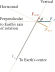
\includegraphics[scale=1]{figures/ch_06/fig_6_5.pdf}
		\caption[]{Thermal vibrations of lattice atoms ($a$ is the amplitude of vibrations, and the shaded circle is effective scattering cross section).}
		\label{fig:6_5}
	\end{center}
	\vspace{-0.7cm}
\end{figure}

Other conditions being equal, the probability for an electron to run into such a disk will, evidently, be proportional to its cross section, and the mean free path of the electron will be inversely proportional to that cross section:
\begin{equation*}
    \lambda \propto \frac{1}{S} \sim \frac{1}{a^2}.
\end{equation*}

The energy of a vibrating atom is proportional to the square of the amplitude: $E\propto a^2$. On the other hand, the average energy of atoms vibrating in a solid is proportional to the absolute temperature of the solid, $T$, that is, $E\propto T$. Therefore, in the high temperature range the mean free path of the electrons due to the thermal lattice vibrations should be inversely proportional to the absolute temperature of the body:
\begin{equation}\label{eq:6_18}
    \lambda \propto \frac{1}{T}.
\end{equation}

This result could have been obtained immediately with the aid of \eqn{4_37}. According to this formula, the phonon concentration in a conductor in the high temperature range is proportional to $T$, that is, $\ab{n}{ph}\propto T$. For electron-phonon scattering, the electron mean free path should evidently be proportional to the phonon concentration and, consequently, inversely proportional to the absolute temperature $T$, that is, $\lambda\propto 1/\ab{n}{ph}\propto 1/T$. On the other hand, the average momentum of a phonon at high temperatures is so great that a single collision of the electron with a phonon (that is, at $\nu\approx 1$) already results in a practically total loss of the electron's initial velocity.

Substituting \eqn{6_18} into Eqs. \eqref{eq:6_5p} and \eqref{eq:6_5pp} and setting $\nu=1$, we obtain the following expressions for the electron mobility:
\begin{align}
    u &\propto \frac{\overline{\lambda}}{\overline{v}} \propto \frac{T^{-1}}{T^{1/2}} = T^{3/2},\quad \text{(nondegenerate gas)} \label{eq:6_19}\\
    u &\propto \frac{\ab{\lambda}{F}}{\ab{v}{F}} \propto \frac{T^{-1}}{\text{constant}} \propto T^{-1}. \quad \text{(degenerate gas)}\label{eq:6_20}
\end{align}

Hence, in the high temperature range, where the dominant effect is scattering by phonons (by the lattice vibrations), the carrier mobility (of electrons or holes) in a nondegenerate gas is inversely proportional to $T^{3/2}$ and in a degenerate gas to $T^{-1}$. We see that in this instance too, the difference in the behaviour of the nondegenerate and the degenerate gases makes itself felt.

\textbf{Low temperature range.} In the low temperature range, the dominant effect is scattering by ionized impurity atoms. The mechanism of the scattering process is such that the impurity ions deflect electrons passing close to them and, thus, reduce their velocities in the original directions. As is shown in \fig{6_6}, the velocity of the electron in the direction of the field was $\vec{v}_0$ before it was deflected by the positively charged ion. After the deflection it fell to $\vec{v}_0'$.

\begin{figure}[t]
	\begin{center}
		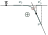
\includegraphics[scale=1]{figures/ch_06/fig_6_6.pdf}
		\caption[]{Electron $q$ scattered by an ionized impurity atom ($\vec{v}_0$ is electron velocity before scattering, and $\vec{v}$ after scattering).}
		\label{fig:6_6}
	\end{center}
	\vspace{-0.7cm}
\end{figure}

The problem of charged centres deflecting charged particles was first solved by E. Rutherford who investigated the scattering of \ce{\alpha}-particles by the nuclei of chemical elements. Applied to our case, the formula for $\nu$ obtained by Rutherford assumes the following form:
\begin{equation}\label{eq:6_21}
    \nu \propto v^4 \parenthesis{\frac{\varepsilon}{Z q}}^2 \ab{m}{n}
\end{equation}

\noindent
where $v$ is the electron velocity, $\varepsilon$ the dielectric constant of the crystal, and $Zq$ the charge of the scattering ion.

This result is quite understandable from qualitative considerations. The higher the electron velocity, their effective mass $\ab{m}{n}$ and the field intensity reduction factor in the crystal (the greater $\varepsilon$ is), the less the electrons will be deflected from their original path and the greater will be the number of collisions needed to randomize electron motion. Evidently, $\nu$ should decrease with the increase in the charge of the scattering ion.

On the other hand, the mean free path of electrons being scattered by ionized impurity atoms is inversely proportional to their concentration and independent of temperature.

Taking this into account and substituting $\nu$ from \eqn{6_21} into Eqs. \eqref{eq:6_5p} and \eqref{eq:6_5pp}, we obtain the following:
\begin{align}
    u &\propto \frac{\overline{\nu}\overline{\lambda}}{\overline{v}} \propto \overline{v}^3 \propto T^{3/2},\quad \text{(nondegenerate gas)} \label{eq:6_22}\\
    u &\propto \frac{\ab{\nu}{F}\ab{\lambda}{F}}{\ab{v}{F}} \propto \ab{v}{F}^3 = \text{constant}. \quad \text{(degenerate gas)}\label{eq:6_23}
\end{align}

Hence, in the low temperature range, the carrier mobility due to scattering by ionized impurity atoms is proportional to $T^{3/2}$ for conductors with a nondegenerate gas, and independent of $T$ for conductors with a degenerate gas.

Figure \ref{fig:6_7}(a) shows the temperature dependence of $u$ for a nondegenerate gas, and \fig{6_7}(b) an experimental $u(T)$ curve for silicon. It follows from \fig{6_7} that experiment, on the whole,
supports the conclusions of the theory as to the nature of the temperature dependence of carrier mobility in nondegenerate conductors.

\begin{figure}[t]
	\begin{center}
		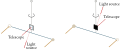
\includegraphics[scale=1]{figures/ch_06/fig_6_7.pdf}
		\caption[]{Temperature dependence of carrier mobility in semiconductors: (a)---theoretical curves; (b)---experimental curves for silicon doped with different amounts of phosphorus.}
		\label{fig:6_7}
	\end{center}
	\vspace{-0.7cm}
\end{figure}

We have discussed the case when in the low temperature range the main effect is due to scattering by ionized impurity atoms. However, for very pure and very perfect metals, containing negligible amounts of impurities and lattice imperfections, phonon scattering may turn out to be the principal charge-carrier scattering mechanism in the low temperature range. Let us find the temperature dependence of $u$ for this case.

For electron-phonon scattering, the electron mean free path $\lambda$ is inversely proportional to the phonon concentration $\ab{n}{ph}$. Since in the low temperature range $\ab{n}{ph}\propto T^3$ according to \eqn{4_36},
\begin{equation}\label{eq:6_24}
	\lambda \propto \frac{1}{\ab{n}{ph}} \propto T^{-3}.
\end{equation}

Now let us determine $\nu$---the average number of collisions the electron should take part in to loose its original directional velocity.

At high temperatures, at which the average phonon momentum $\ab{p}{ph}$ is equal, in order of magnitude, to the electron momentum $\ab{p}{e}$, $\nu\approx 1$. At low temperatures, $\ab{p}{ph}\ll\ab{p}{e}$, and as a result $\nu$ can be much greater than unity, being substantially dependent on temperature since $\ab{p}{ph}$ rises with the rise in $T$.

Figure \ref{fig:6_8} shows the variation of the momentum of an electron that took part in an elastic collision with a phonon. The collision took place at point A. Before the collision, the electron's momentum was $\ab{\vec{p}}{e}^0$ and after the collision it became $\ab{\vec{p}}{e}$. Since the collision was an elastic one, the absolute value of the momentum has not changed: $\ab{p}{e}^0=\ab{p}{e}$. Only the direction has changed so that
\begin{equation*}
	\ab{\vec{p}}{e} = \ab{\vec{p}}{e}^0 + \ab{\vec{p}}{ph}.
\end{equation*}

\begin{figure}[t]
	\begin{center}
		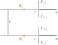
\includegraphics[scale=1]{figures/ch_06/fig_6_8.pdf}
		\caption[]{Calculating the number of collisions needed to nullify the electron's momentum in a given direction.}
		\label{fig:6_8}
	\end{center}
	\vspace{-0.7cm}
\end{figure}

The change in the direction of the electron's momentum brought about by the collision entails a reduction in its value in the original direction by $\Delta{\ab{p}{e}}$ (\fig{6_8}). It follows from $\Delta$BCD that
\begin{equation*}
	\Delta{\ab{p}{e}} = \ab{p}{ph} \sin\parenthesis{\frac{\varphi}{2}}
\end{equation*}

\noindent
where $\varphi$ is the electron scattering angle. From $\Delta$AEC, it follows that $\sin(\varphi/2)=\ab{p}{ph}/(2\ab{p}{e})$. Therefore,
\begin{equation*}
	\Delta{\ab{p}{e}} = \frac{\ab{p}{ph}^2}{2\ab{p}{e}}.
\end{equation*}

\noindent
It is by this quantity that the electron momentum, in the original direction, is reduced as a result of a single collision with a phonon. To eliminate the electron momentum in the original direction altogether, the following number of collisions is needed:
\begin{equation*}
	\nu \approx \frac{\ab{p}{e}}{\Delta{\ab{p}{e}}} \approx 2 \parenthesis{\frac{\ab{p}{e}}{\ab{p}{ph}}}^2 \propto \frac{1}{\ab{p}{ph}^2}.
\end{equation*}

In the low temperature range, the energy of thermal lattice vibrations (the phonon gas energy) is, according to Eqs. \eqref{eq:4_30} and \eqref{eq:4_36}, $\ab{E}{lattice}\propto T^4$ and the phonon gas concentration is $\ab{n}{ph}\propto T^3$. Therefore, the average phonon energy
\begin{equation*}
	\ab{\overline{\varepsilon}}{ph} = \frac{\ab{E}{lattice}}{\ab{n}{ph}} \propto T
\end{equation*}

\noindent
increases in proportion to $T$. Since the phonon momentum is
\begin{equation*}
	\ab{p}{ph} = \frac{\ab{\overline{\varepsilon}}{ph}}{v}
\end{equation*}

\noindent
($v$ is the velocity of sound in the crystal), the phonon momentum in this temperature range is also proportional to $T$:
\begin{equation}\label{eq:6_25}
	\ab{p}{ph} \propto T.
\end{equation}

\noindent
Therefore,
\begin{equation}\label{eq:6_26}
	\nu \propto \frac{1}{\ab{p}{ph}^2} \propto T^{-2}.
\end{equation}

\noindent
Substituting $\lambda$, from \eqn{6_24} and $\nu$ from \eqn{6_26} into \eqn{6_5pp}, we obtain the following expression for free carrier mobility in pure metals in the low temperature range:
\begin{equation}\label{eq:6_27}
	u \propto \frac{\ab{\nu}{F} \ab{\lambda}{F}}{\ab{v}{F}} \propto T^{-5}.
\end{equation}

Figure \ref{fig:6_9} shows the qualitative curve of the temperature dependence of $u$ for pure metals. In the high temperature range (above the Debye temperature $\Theta$) the carrier mobility $u\propto T^{-1}$, in the low temperature range (much below $\Theta$) $u\propto T^{-5}$. In the intermediate temperature
range, a gradual transition from the $T^{-1}$ to the $T^{-5}$ dependence takes place. Finally, close to absolute zero, the thermal vibrations become so weak that carrier scattering by impurity atoms and lattice defects, which are always present in a metal no matter how pure and perfect it is, becomes of primary importance. In this case, the carrier mobility ceases to depend on temperature [see \eqn{6_23}] and the $u$ versus $T$ curve follows a line parallel to the temperature axis.

\begin{figure}[t]
	\begin{center}
		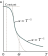
\includegraphics[scale=1]{figures/ch_06/fig_6_9.pdf}
		\caption[]{Temperature dependence of free electron mobility in pure metals.}
		\label{fig:6_9}
	\end{center}
	\vspace{-0.7cm}
\end{figure}

\section{Electrical conductivity of pure metals}\label{sec:54}

Electrical conductivity of pure metals is due to the drift of free charge carriers of one sign. In the absolute majority of pure metals, the charge carriers are free electrons. However, in some metals, such as beryllium and zinc, the charge is carried by holes.

The conductivity, or specific conductance, of electron metals is described by \eqn{6_12}:
\begin{equation*}
	\sigma = qnu.
\end{equation*}

\noindent
Since the metals are degenerate conductors, the electron concentration in them is practically independent of temperature. Because of that, temperature dependence of specific conductance is determined entirely by the temperature dependence of the mobility of the electrons in a degenerate electron gas, as discussed in the previous section.

Substituting $u$ from Eqs. \eqref{eq:6_20} and \eqref{eq:6_27} into \eqref{eq:6_12}, we obtain the
following expression for $\sigma$ and the specific resistance $\rho$ of pure metals:
\begin{align}
	\sigma &= \frac{A}{T},\quad \rho = a T,\quad \text{(high temperature range)}\label{eq:6_28}\\
	\sigma &= \frac{B}{T^5},\quad \rho = b T^5.\quad \text{(low temperature range)}\label{eq:6_29}
\end{align}

\noindent
Here, $A$, $B$, $a$, and $b$ are proportionality factors.

\begin{figure}[t]
	\begin{center}
		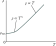
\includegraphics[scale=1]{figures/ch_06/fig_6_10.pdf}
		\caption[]{Schematic plot of the temperature dependence of specific resistance of pure metals.}
		\label{fig:6_10}
	\end{center}
	\vspace{-0.7cm}
\end{figure}

Figure \ref{fig:6_10} shows schematically the dependence of specific resistance of pure metals on temperature. In the high temperature range, this dependence is represented by a straight line, in the low temperature range, by a parabola of the fifth degree, and in the vicinity of absolute zero, by a straight line parallel to the temperature axis.

A more rigorous quantum mechanical calculation enables the coefficients $A$, $B$, $a$ and $b$ in formulae \eqref{eq:6_28} and \eqref{eq:6_29} to be found. Table \ref{table:6_2} shows the specific conductance of some pure metals at room temperature, calculated ($\ab{\sigma}{theory}$) and measured experimentally ($\ab{\sigma}{experiment}$) (in units of \SI{e6}{\per\ohm\per\metre}).

It follows that for Na and K, in which the conducting electrons are almost in a free state, the agreement between theory and experiment is satisfactory. As the atomic mass increases, so does the lattice potential and the interaction of the conducting electrons with the
lattice. This means that the free electron approximation becomes less valid. The result is a discrepancy between $\ab{\sigma}{theory}$ and $\ab{\sigma}{experiment}$ which grows.

Table \ref{table:6_3} shows the ratios of the specific conductivity of gold $\sigma_0$ at \SI{273}{\kelvin} to $\sigma$ at low temperatures, calculated and measured.

The agreement between theory and experiment seems to be quite satisfactory.

\begin{table}[!b]
	\renewcommand{\arraystretch}{1.2}
	\caption{}
	\vspace{-0.6cm}
	\label{table:6_2}
	\begin{center}\resizebox{0.58\linewidth}{!}{
			\begin{tabular}{lcccccc}
				\toprule[1pt]
                & Na & K & Rb & Cu & Ag & Au\\
                \midrule[0.5pt]\midrule[0.5pt]
                $\ab{\sigma}{theory}$ & $22$ & $19$ & $20$ & $100$ & $90$ & $107$\\
				$\ab{\sigma}{experiment}$ & $23$ & $15$ & $8$ & $64$ & $67$ & $68$\\
				\bottomrule[1pt]
			\end{tabular}
	}\end{center}
\end{table}

\begin{table}[!b]
	\renewcommand{\arraystretch}{1.2}
	\caption{}
	\vspace{-0.6cm}
	\label{table:6_3}
	\begin{center}\resizebox{0.95\linewidth}{!}{
			\begin{tabular}{lcccccc}
				\toprule[1pt]
                & \SI{273}{\kelvin} & \SI{87.4}{\kelvin} & \SI{57.8}{\kelvin} & \SI{20.4}{\kelvin} & \SI{11.1}{\kelvin} & \SI{4.2}{\kelvin}\\
                \midrule[0.5pt]\midrule[0.5pt]
                $(\sigma_0/\sigma)_{\text{theory}}$ & $1$ & $0.2645$ & $0.1356$ & $0.0060$ & $0.0003$ & \num{3e-6}\\
				$(\sigma_0/\sigma)_{\text{experiment}}$ & $1$ & $0.2551$ & $0.1314$ & $0.0058$ & $0.0003$ & \num{3e-6}\\
				\bottomrule[1pt]
			\end{tabular}
	}\end{center}
\end{table}

\section{Electrical conductivity of metal alloys}\label{sec:55}

In metal alloys too, the carrier concentration is independent of temperature. Therefore, the temperature dependence of specific conductance in alloys is determined entirely by the temperature dependence of the carrier mobility. Let us discuss this problem in more detail.

Suppose that some sites of an ideal metal lattice, for instance, of a copper lattice, with a strictly periodic potential [\fig{6_11}(a)] are at random replaced by atoms of some other element, say, gold. Since the potential of the field of an impurity atom is not the same as that of the matrix atom, the lattice potential will cease to be strictly periodic [\fig{6_11}(b)]. It will be distorted by the disordered impurity atoms. Naturally, such distortion will lead to carrier scattering and to the appearance of additional electrical resistance.

\begin{figure}[t]
	\begin{center}
		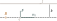
\includegraphics[scale=1]{figures/ch_06/fig_6_11.pdf}
		\caption[]{Violation of lattice potential's periodicity by impurity atoms: (a)---strictly periodic potential of ideal lattice built of atoms of one kind; (b)---violation of potential's periodicity by impurity atoms substituting matrix atoms at random.}
		\label{fig:6_11}
	\end{center}
	\vspace{-0.7cm}
\end{figure}

It was L. Nordheim who demonstrated that, in the simplest case of binary alloys of the solid solution type, the carrier mobility due to scattering on lattice imperfections is described by the following approximate relation:
\begin{equation}\label{eq:6_30}
	\ab{u}{al} \propto \omega (1-\omega)
\end{equation}

\noindent
where $\omega$ and $(1-\omega)$ are the fractional parts of the metals constituting the alloy.

Substituting $\ab{u}{al}$ from \eqn{6_30} into \eqn{6_12} and keeping in mind that $\rho=1/\sigma$, we obtain the following expression for the specific resistance of a binary alloy:
\begin{equation}\label{eq:6_31}
	\ab{\rho}{al} = \beta [\omega (1-\omega)]
\end{equation}

\noindent
where $\beta$ is a proportionality factor.

The function $\omega (1-\omega)$ has a maximum at $\omega=1/2$, that is when the concentrations of both components are equal. Figure \ref{fig:6_12}(a) shows the dependence of the specific resistance of copper-gold alloys on the gold contents. The curve passes through a maximum corresponding to a $50\%$ contents of copper (or gold) in the alloy.

It also follows from \fig{6_12}(a) that $\ab{rho}{al}$ is much greater than that of the pure components. For instance, at room temperature, $\ab{\rho}{Cu}=\SI{1.7e-8}{\ohm\metre}$ and $\ab{\rho}{Au}=\SI{1.56e-8}{\ohm\metre}$, whereas $\ab{\rho}{$50\%$Cu$+50\%$Au}=\SI{15e-8}{\ohm\metre}$. This is quite natural since the disorder in the lattice has a much more detrimental effect on the lattice periodicity than the thermal vibrations.
If, however, the alloyed metals taken in appropriate proportions form ordered alloys, or metallic compounds, with an ordered structure, the lattice periodicity is recovered [\fig{6_12}(b)] and the resistance due to impurity scattering vanishes practically altogether. For the copper-gold alloys, the appropriate concentrations are those which correspond to the stoichiometric composition of \ce{Cu3Au} and \ce{CuAu} [\fig{6_12}(a), solid curves]. This may serve as a proof of the validity of the quantum theory of electrical conductivity, which maintains that the cause of the electrical resistance of solids is not the collision of the free electrons with the lattice atoms but their scattering by the lattice defects which distort the periodic lattice potential. An ideal regular imperfection-free lattice with a strictly periodic potential is incapable of scattering free charge carriers and must therefore have zero resistance. This conclusion is supported by numerous experiments carried out with extremely pure metals in the low temperature range, the relevant data being presented in \tab{6_3}: as the degree of purity of a metal is increased its specific resistance near absolute zero diminishes, continuously tending to zero. We would like to stress that, this is not the phenomenon of superconductivity which we shall discuss later, but the natural behaviour of absolutely all pure metals in the extreme low temperature range, which is a consequence of the quantum mechanical nature of electrical resistance.

\begin{figure}[t]
	\begin{center}
		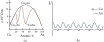
\includegraphics[scale=1]{figures/ch_06/fig_6_12.pdf}
		\caption[]{(a)---dependence of specific resistance of solid solutions of gold and copper on composition, (b)---lattice potential's periodicity recovered in the ordering of the structure.}
		\label{fig:6_12}
	\end{center}
	\vspace{-0.7cm}
\end{figure}

For small impurity contents one may set in \eqn{6_31} $(1-\omega)\approx 1$. Then, $\ab{p}{al}\propto\omega$. This specific resistance is independent of temperature and does not vanish at absolute zero. It is termed \textit{residual resistivity} $\ab{\rho}{res}$ (see \fig{6_10}).

At temperatures other than absolute zero, a resistivity $\ab{\rho}{T}$ due to electron scattering by the lattice vibrations is added to the residual resistivity and the total resistivity becomes
\begin{equation}\label{eq:6_32}
	\rho = \ab{\rho}{res} + \ab{\rho}{T}.
\end{equation}

\noindent
This relation expresses \textit{Matthiessen's rule}, which speaks of the additivity of specific resistance.

Let us discuss now the \textit{temperature coefficient of resistivity} $\alpha$. As is well known, it expresses the relative variation of the specific resistance of a conductor whose temperature is raised by \SI{1}{\kelvin}. For pure metals, $\rho = \ab{\rho}{T}$ and therefore,
\begin{equation}\label{eq:6_33}
	\alpha = \frac{1}{\ab{\rho}{T}}\, \diff{\ab{\rho}{T}}{T}.
\end{equation}

Experiment shows $\alpha$ roughly to be
\begin{equation*}
	\alpha \approx \frac{1}{273}\, \si{\per\kelvin} \approx \SI{0.004}{\per\kelvin}
\end{equation*}

\noindent
[see \tab{6_4}]. For alloys, $\rho=\ab{\rho}{res}+\ab{\rho}{T}$; therefore,
\begin{equation*}
	\ab{\alpha}{al} = \frac{1}{\rho}\, \diff{\rho}{T} = \frac{1}{\parenthesis{\ab{\rho}{res}+\ab{\rho}{T}}}\, \diff{\ab{\rho}{T}}{T}
\end{equation*}

\noindent
since $\ab{\rho}{res}$ is independent of temperature. This expression may be transformed into
\begin{equation}\label{eq:6_34}
	\ab{\alpha}{al} = \frac{1}{\parenthesis{1 + \dfrac{\ab{\rho}{res}}{\ab{\rho}{T}}}} \frac{1}{\ab{\rho}{T}}\, \diff{\ab{\rho}{T}}{T} = \frac{\alpha}{\parenthesis{1 + \dfrac{\ab{\rho}{res}}{\ab{\rho}{T}}}}
\end{equation}

\noindent
where $\alpha$ is the temperature coefficient of resistivity of pure metals.

It follows from \eqn{6_34} that $\ab{\alpha}{al}$ should be less than $\alpha$ of a pure metal, the less the greater $\ab{\rho}{res}$ is in comparison with $\ab{\rho}{T}$. Usually, $\ab{\rho}{res}$ is an order of magnitude or more greater than $\ab{\rho}{T}$. Therefore, $\ab{\alpha}{al}$ may be an order of magnitude or less than $\alpha$ of a pure metal, and this is on the whole supported by experiment (\tab{6_4}; the data are for room temperature).

\begin{table}[!b]
	\renewcommand{\arraystretch}{1.2}
	\caption{}
	\vspace{-0.6cm}
	\label{table:6_4}
	\begin{center}\resizebox{0.88\linewidth}{!}{
			\begin{tabular}{lccclll}
				\toprule[1pt]
                & & & & Bronze & Nichrome & Constantan\\
				& Cu & Sn & Ni & ($88\%$ Cu, & ($80\%$ Ni, & ($54\%$ Cu,\\
				& & & & $18\%$ Sn, $1\%$ Pb) & $20\%$ Cr) & $46\%$ Ni)\\
                \midrule[0.5pt]\midrule[0.5pt]
                $\alpha$ (\SI{e3}{\per\kelvin}) & $4.1$ & $4.2$ & $6.2$ & $0.5$ & $0.13$ & $-0.004$\\
				\bottomrule[1pt]
			\end{tabular}
	}\end{center}
\end{table}

However, in many cases, the temperature dependence of an alloy's resistance is much more complex than that which follows from the simple additive rule \eqref{eq:6_32}, and the temperature coefficient of resistivity of some alloys may be much less than one could expect from \eqn{6_34}. More than that, it does not remain constant in a wide temperature interval but may in some cases even become negative as is, for instance, the case with constantan (\tab{6_4}) and with some other alloys.

A high specific resistance together with a low temperature coefficient of resistivity made alloys valuable materials for the production of various wire and film resistors and variable resistors (rheostats) widely used in different fields of science and technology.

\section{Intrinsic conductivity of semiconductors}\label{sec:56}

The electrical conductivity of very pure and perfect single crystal semiconductors, in the not very low temperature range, is due to intrinsic charge carriers, that is, to electrons and holes. Such conductivity is termed \textit{intrinsic}.

Since there are two types of carriers in the intrinsic semiconductor, electrons and holes, its specific conductance is the sum of the conductivity $\ab{\sigma}{n}=q\ab{n}{i}\ab{u}{n}$ due to free electrons, with the concentration $\ab{n}{i}$ and the mobility $\ab{u}{n}$, and of the conductivity $\ab{\sigma}{p}=q\ab{p}{i}\ab{u}{p}$ due to
the presence of holes, with the concentration $\ab{p}{i}$ and the mobility $\ab{u}{p}$. Since $\ab{n}{i}=\ab{p}{i}$, the total specific conductance of an intrinsic semiconductor is
\begin{equation}\label{eq:6_35}
	\ab{\sigma}{i} = \ab{\sigma}{n} + \ab{\sigma}{p} = q \ab{n}{i} (\ab{u}{n} + \ab{u}{p}).
\end{equation}

According to \eqn{5_37}, the hole (or electron) concentration in an intrinsic semiconductor is
\begin{equation*}
	\ab{n}{i} = \ab{p}{i} = 2 \parenthesis{\frac{2 \pi \sqrt{\ab{m}{n} \ab{m}{p}} \ab{k}{B} T}{h^2}}^{3/2} e^{-\ab{E}{g}/(2\ab{k}{B}T)}.
\end{equation*}

\noindent
The carrier mobility in the intrinsic conductivity range is given by \eqn{6_19}. Substituting Eqs. \eqref{eq:5_37} and \eqref{eq:6_19} into \eqref{eq:6_35} we obtain
\begin{equation}\label{eq:6_36}
	\ab{\sigma}{i} = \sigma_0\, e^{-\ab{E}{g}/(2\ab{k}{B}T)}
\end{equation}

\noindent
where $\sigma_0$ denotes the preexponential expression.

It follows from \eqn{6_36} that, $\ab{\sigma}{i}\to \sigma_0$ as $T\to\infty$. We thus conclude that, if the rule \eqref{eq:6_36} remains valid for infinitely high temperatures, $\sigma_0$ would be the specific conductance of the semiconductor as $T\to\infty$.

The temperature dependence of $\ab{\sigma}{i}$ can be conveniently represented in the semilogarithmic coordinates. Taking the logarithm of \eqn{6_36}, we obtain
\begin{equation}\label{eq:6_37}
	\ln{\ab{\sigma}{i}} = \ln{\sigma_0} - \parenthesis{\frac{\ab{E}{g}}{2\ab{k}{B}T}}.
\end{equation}

\noindent
If we plot $1/T$ along the $x$ axis and $\ln{\sigma}$ along the $y$ axis, we will obtain a straight line that cuts off a section $\ln{\sigma_0}$ [\fig{6_13}(a)] on the $y$ axis. The tangent of $\alpha$ of this straight line to the $x$ axis is equal to $\ab{E}{g}/(2\ab{k}{B}T)$. Plotting this dependence, we can find the constant $\sigma_0$ and the width of the forbidden band $\ab{E}{g}$.
Figure \ref{fig:6_13}(b) shows the experimental $\ln{\ab{\sigma}{i}}$ versus $1/T$ dependence for pure germanium and silicon. The forbidden bands as determined from the inclination angles of the curves turned out to be \SI{0.72}{\electronvolt} and \SI{1.2}{\electronvolt} wide.

\begin{figure}[t]
	\begin{center}
		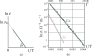
\includegraphics[scale=1]{figures/ch_06/fig_6_13.pdf}
		\caption[]{Temperature dependence of intrinsic conductivity of a semiconductor: (a)---theoretical curve; (b)---experimental plots for germanium and silicon.}
		\label{fig:6_13}
	\end{center}
	\vspace{-0.7cm}
\end{figure}

Comparing the results of this section with those of the previous one, we see that there is the following principal difference between metals and semiconductors. In metals, where the electron gas is in a degenerate state, the carrier concentration is practically independent of temperature and the temperature dependence of conductivity is determined entirely by the temperature dependence of carrier mobility. In the semiconductors, on the other hand, the carrier gas is nondegenerate and its concentration depends strongly on temperature [see \eqn{5_37}]. Because of that, their conductivity is entirely determined by the temperature dependence of carrier concentration [see \eqn{6_36}].

For a specific temperature the carrier concentration and the conductivity of a semiconductor are determined by the width of its forbidden band. This may be seen quite clearly from the data of \tab{6_5}
which contains the widths of the forbidden bands and the specific resistances of the elements of Group IV of the Mendeleev periodic table, the elements having the diamond-type lattice. As the width of the forbidden band decreases from \SI{5.2}{\electronvolt} (diamond) to \SI{0.08}{\electronvolt} (gray tin), the room temperature specific resistance diminishes by $16$ orders of magnitude.

\begin{table}[!b]
	\renewcommand{\arraystretch}{1.2}
	\caption{}
	\vspace{-0.6cm}
	\label{table:6_5}
	\begin{center}\resizebox{0.7\linewidth}{!}{
			\begin{tabular}{lcccc}
				\toprule[1pt]
                & Diamond & Silicon & Germanium & Gray tin\\
                \midrule[0.5pt]\midrule[0.5pt]
                $\ab{E}{g}$ (\si{\electronvolt}) & $5.2$ & $1.12$ & $0.66$ & $0.08$\\
				$\rho$ (\si{\ohm\metre}) & \num{e10} & \num{3e3} & $0.47$ & \num{2e-6}\\
				\bottomrule[1pt]
			\end{tabular}
	}\end{center}
\end{table}

\section{Impurity (extrinsic) conductivity of semiconductors}\label{sec:57}

The temperature dependence of specific conductance of nondegenerate impurity semiconductors, as that of intrinsic semiconductors, is for the most part determined by the temperature dependence of carrier concentration. Because of this, the curve representing the temperature dependence of $\sigma$ must at least qualitatively be analogous to the $n$ versus $T$ curve, where the latter is shown in \fig{5_22}.

The temperature dependence of $\ln{\sigma}$ for an impurity semiconductor is represented qualitatively in \fig{6_14}(a). There are three distinct regions on this curve ab, be, and cd.

\begin{figure}[t]
	\begin{center}
		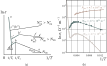
\includegraphics[scale=1]{figures/ch_06/fig_6_14.pdf}
		\caption[]{Temperature dependence of specific conductance of impurity: semiconductors: (a)---theoretical curve; (b)---experimental plots for silicon containing different amounts of phosphorus.}
		\label{fig:6_14}
	\end{center}
	\vspace{-0.7cm}
\end{figure}

The region ab lies between absolute zero and the impurity saturation temperature $\ab{T}{s}$. The carrier concentration in this region is described by \eqn{5_41}:
\begin{equation*}
	n = \sqrt{2 \ab{N}{d}} \parenthesis{\frac{2 \pi \ab{m}{n} \ab{k}{B} T}{h^2}}^{3/2} e^{-\ab{E}{d}/(2\ab{k}{B}T)}.
\end{equation*}

\noindent
The mobility is determined mainly by impurity and imperfection scattering, and according to \eqn{6_22}, is proportional to $T^{3/2}$. Substituting Eqs. \eqref{eq:5_41} and \eqref{eq:6_22} into \eqref{eq:6_12} we obtain
\begin{equation}\label{eq:6_38}
	\ab{\sigma}{im} = \ab{\sigma}{im}^0\, e^{-\ab{E}{d}/(2\ab{k}{B}T)}
\end{equation}

\noindent
where $\ab{\sigma}{im}^0$ is a factor that depends weakly on temperature (as compared with the exponential).

Taking the logarithm of \eqn{6_38}, we obtain
\begin{equation}\label{eq:6_39}
	\ln{\ab{\sigma}{im}} = \ln{\ab{\sigma}{im}^0} - \parenthesis{\frac{\ab{E}{d}}{2\ab{k}{B}T}}.
\end{equation}

\noindent
In the $\ln{\ab{\sigma}{im}}$ versus $1/T$ coordinate system we get a straight line which makes an angle $\ab{\alpha}{im}$ with the $1/T$ axis such that tan $\ab{\alpha}{im}=\ab{E}{d}/(2\ab{k}{B})$ is proportional to the impurity ionization energy $\ab{E}{d}$. Hence, region ab corresponds to impurity, or extrinsic, conductivity, which is due to impurity carriers freed as the result of the ionization of impurity atoms.

The region bc lies between the impurity saturation temperature $\ab{T}{a}$ and the temperature of intrinsic conductivity $\ab{T}{i}$. In this range, all the impurity atoms are ionized but no noticeable excitation of intrinsic carriers takes place. Because of that, the carrier concentration remains approximately constant and equal to the impurity concentration $n\approx\ab{N}{d}$. Therefore, in this region the temperature dependence of the conductivity is determined by the temperature dependence of carrier mobility. If the principal carrier scattering mechanism inside this region is the scattering on thermal lattice vibrations, which causes the mobility to fall with temperature, then the specific conductance will also diminish with the rise in temperature. This is just the case shown in \fig{6_14}(a). But if the principal mechanism is impurity or imperfection scattering, then the specific conductance in the region bc will increase with temperature.

The region cd corresponds to the transition to intrinsic conductivity. Inside this region, the carrier concentration is equal to the intrinsic carrier concentration. Therefore, the conductivity of the semiconductor in this region is
\begin{equation*}
	\sigma \approx \ab{\sigma}{im} = \ab{\sigma}{im}^0\, e^{-\ab{E}{d}/(2\ab{k}{B}T)}.
\end{equation*}

\noindent
In semilogarithmic coordinates $\ln{\sigma}$ versus $1/T$ this dependence is represented by a straight line cd, making an angle $\ab{\alpha}{i}$ with the $1/T$ axis, its tangent being proportional to the width of the forbidden band: $\tan\ab{\alpha}{i}=\ab{E}{d}/(2\ab{k}{B})$.

Figure \ref{fig:6_14}(b) shows the temperature dependence of the conductivity of phos-phorus-doped silicon. A comparison with \fig{6_14}(a) shows that in the simplest cases the theory ensures a qualitative agreement with experiment.

\textbf{Thermistors.} The strong dependence of the resistance of semiconductors on the temperature is utilized in a wide class of semiconductor devices, the thermistors. They are bulk semiconductor resistors with a large temperature coefficient of resistivity and a nonlinear current-voltage characteristic.

Thermistors are used in measuring temperature and power of ultrahigh frequency radiation, for temperature compensation in various electric circuits, for timing relays, etc. Microthermistors, which have small dimensions and low thermal inertia, are being used in the study of heat exchange processes in plants and living organisms including early diagnosis of human illnesses. The use of a thin semiconducting film in a bolometer, made it possible to increase its sensitivity to \SI{e-10}{\watt}. Such bolometers placed in the focus of a parabolic mirror are capable of detecting aircraft, tanks, ships and other bodies that radiate heat at a distance of the order of several kilometers. A highly sensitive semiconductor bolometer detected infrared radiation reflected by the moon's surface.

\section{Deviation from Ohm's law. The effect of a strong field}\label{sec:58}

The proportionality between the current density $\vec{i}$ and the field intensity $\vec{\mathcal{E}}$ demanded by the Ohm's law \eqref{eq:6_1} remains as long as $\sigma$, which enters this law as a proportionality factor, remains independent of $\vec{\mathcal{E}}$.

Let us find what are the conditions in which this requirement is fulfilled.

According to \eqn{6_5p}, the carrier mobility in nondegenerate semiconductors $u\propto\lambda/v$, where $v$ is the resultant velocity of carrier motion. It is the sum of the thermal $v_0$ and drift $\ab{v}{d}$ velocities:
\begin{equation*}
	\vec{v} = \vec{v}_0 + \ab{\vec{v}}{d}.
\end{equation*}

\noindent
For weak fields
\begin{equation}\label{eq:6_40}
	\ab{v}{d} \ll v_0
\end{equation}

\noindent
the resultant carrier velocity is $v_0$ and is independent of $\mathcal{E}$. Therefore, both the carrier mobility $u$ and their concentration and,
consequently, the specific conductance $\sigma=qnu$ are independent of $\mathcal{E}$. Such fields are termed \textit{weak}.

Hence, Ohm's law, which requires a linear dependence of $\vec{i}$ on $\vec{\mathcal{E}}$, is valid only in the case of weak fields complying with the condition \eqref{eq:6_40}.

As the field $\vec{\mathcal{E}}$ increases, the drift velocity $\ab{v}{d}$ rises, and in fields of high intensity, may become comparable in order of magnitude with $v_0$. In this case, the resultant velocity begins to be dependent on $\vec{\mathcal{E}}$ and because of that, the mobility $u$ and the specific conductance $\sigma$ too become dependent on $\vec{\mathcal{E}}$. Naturally, the result is a distortion of the linear
dependence of $\vec{i}$ on $\vec{\mathcal{E}}$, that is, a deviation from Ohm's law. Fields in which such phenomena take place are termed \textit{strong}.

Calculations show that when scattering by thermal lattice vibrations is the principal scattering mechanism in strong fields
\begin{equation}\label{eq:6_41}
	u \propto \mathcal{E}^{-1/2},\quad \sigma = qnu \propto\mathcal{E}^{-1/2},\quad i = \sigma\mathcal{E} \propto \mathcal{E}^{1/2}.
\end{equation}

In still stronger fields, the drift velocity $\ab{v}{d}$ ceases to be dependent on the so-called \textit{drift velocity saturation effect} sets in (\fig{6_15}). Since $i\propto\ab{v}{d}$, such fields are also characterized by current saturation. The current-voltage characteristic of a semiconductor becomes distinctly nonlinear.

\begin{figure}[t]
	\begin{center}
		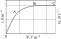
\includegraphics[scale=1]{figures/ch_06/fig_6_15.pdf}
		\caption[]{Nonlinear carrier drift velocity in semiconductors: $i\propto\mathcal{E}$ (Ohm's law) in region $0$A, $i\propto\sqrt{\mathcal{E}}$ in region AB, and $i$ is independent of $\mathcal{E}$ in region BC (saturation of drift velocity).}
		\label{fig:6_15}
	\end{center}
	\vspace{-0.7cm}
\end{figure}

The rise in the resultant electron velocity in an external field is equivalent to the rise in the temperature of the electron gas. Therefore, this effect is known as electron gas heating and the electrons whose average kinetic energy exceeds that of the lattice atoms are termed \textit{hot electrons}.

Strong fields can bring about not only changes in carrier mobility but in their concentration as well. There are several mechanisms leading to that result.

\textbf{Thermoelectron ionization.} In strong fields, not only free electrons become heated but to a lesser extent, bound electrons too. Therefore, the probability of their transition to the conduction band increases in the same way as it would increase if the temperature of the semiconductor as a whole would be raised by an appropriate amount. This results in an increase in free carrier concentration and in the specific conductance of the semiconductor, $\sigma$. Such phenomenon became known by the name of \textit{thermoelectron ionization}. Its theory was developed by Ya. I. Frenkel.

\textbf{Impact ionization.} If conduction electrons of a heated electron gas receive enough energy to ionize neutral atoms lifting their electrons to the conduction band and themselves remaining in the conduction band, then there will be an avalanche-type increase in the free carrier concentration, until the process is counterbalanced by recombination. This mechanism of free carrier breeding is termed \textit{impact ionization}.

\textbf{Electrostatic ionization.} In high-intensity fields the transition of the electrons from the valence band to the conduction band by means of tunnelling through the forbidden band becomes possible. This effect is known as the \textit{Zener effect}, or \textit{electrostatic ionization}. The probability of tunnelling and, consequently, the tunnel current density increase drastically with the increase in the field intensity and decrease with the increase in the width of the forbidden band.

Figure \ref{fig:6_16} shows a qualitative curve of the variation of specific conductance of germanium with field intensity (in semilogarithmic approximate coordinates). Also shown are limits within which those mechanisms of carrier generation resulting in the increase in electric conductivity operate ($1,2$---the ohmic and the Frenkel regions; $3,4$---the regions of electrostatic ionization and breakdown).

\begin{figure}[t]
	\begin{center}
		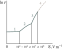
\includegraphics[scale=1]{figures/ch_06/fig_6_16.pdf}
		\caption[]{Qualitative dependence of specific conductance of germanium on electric field intensity: $1$---ohmic region, $2$---Frenkel region, $3$---electrostatic ionization region, $4$---breakdown region.}
		\label{fig:6_16}
	\end{center}
	\vspace{-0.7cm}
\end{figure}

\section{The Gunn effect}\label{sec:59}

It was demonstrated in the previous section that in strong fields there is a phenomenon of nonlinear drift velocity: the drift velocity changes not in direct proportion to the field intensity $\vec{\mathcal{E}}$, the result being a deviation from Ohm's law.

An interesting effect of nonlinear drift velocity in gallium arsenide was discovered by J. B. Gunn. It became known as the \textit{Gunn effect}. Figure \ref{fig:6_17}(a) shows the pattern of the conduction band of gallium arsenide. It has two minimums in the $[100]$ direction: one at $k=0$ and the other at $k=0.8k_0$ ($k_0$ is the wave vector corresponding to the Brillouin zone boundary). The second minimum is $E=\SI{0.36}{\electronvolt}$ above the first. In normal conditions the electrons of the conduction band occupy the first minimum, where their effective mass is $\ab{m}{n}'=0.072m$ and the mobility $u_1=\SI{0.5}{\volt\per\metre\squared\per\second}$.
When an external field is applied to the crystal, the electrons' drift velocity becomes $\ab{v}{d}'=u_1\mathcal{E}$, which increases in proportion to $\mathcal{E}$ [the straight line $0$A,
\fig{6_17}(b)]. This goes on until the heated electrons accumulate sufficient energy to go over to the upper minimum, where their effective mass is much greater ($\ab{m}{n}''=1.2m$) and the mobility much lower ($u_2=\SI{0.01}{\volt\per\metre\squared\per\second}$). Such a transition results in a drastic reduction in the drift velocity (because of a lower electron mobility) and the current density, that is, in the appearance of the region AB with a negative differential conductivity ($\ab{\sigma}{dif}=\diffin{i}{V}$). After most of the
electrons move over to the upper minimum any further, increase in $\mathcal{E}$ will be accompanied by an increase in drift velocity $\ab{v}{d}''=u_2\mathcal{E}$ and by a proportional increase in the current density $i$ (region BC).

The presence of a negative differential conductivity region on the current-voltage characteristic of a gallium arsenide crystal makes it possible to devise, on the basis of the Gunn effect, ultra-high frequency (UHF) oscillators known as \textit{Gunn diodes}.

\begin{figure}[t]
	\begin{center}
		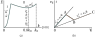
\includegraphics[scale=1]{figures/ch_06/fig_6_17.pdf}
		\caption[]{The Gunn effect: (a)---structure of conduction band in allium arsenide in $[100]$ direction; (b)---variation of drift velocity and current density with the increase in electric field intensity.}
		\label{fig:6_17}
	\end{center}
	\vspace{-0.7cm}
\end{figure}

The Gunn effect was first discovered in 1963. In 1966, a first commercial type of an UHF generator working at a frequency of \SIrange{2}{3}{\giga\hertz}
with a power output of approximately \SI{100}{\watt} in pulsed operation, was produced. At an electronic instrumentation and automatics exhibition which took place in the United States in 1968, radars using Gunn generators to measure the speed of moving objects were displayed. Those radars were so small that they could be carried by hand.

\section{Photoconductivity of semiconductors}\label{sec:60}

Let us turn a ray of light of intensity $I_0$ on the semiconductor [\fig{6_18}(a)]. Passing through the semiconductor the light is gradually absorbed and its intensity is diminished. Cut out an infinitely thin layer $\deriv{x}$ at a distance $x$ from the semiconductor's surface. The amount of luminous energy $\deriv{J}$ absorbed in the layer $\deriv{x}$ is proportional to the intensity $J$ of the light passing through this layer and to its thickness $\deriv{x}$:
\begin{equation}\label{eq:6_42}
	\deriv{J} = -kJ\, \deriv{x}.
\end{equation}

\noindent
The minus sign shows that the energy diminishes; the term for the proportionality factor $k$ is \textit{absorption coefficient}. For $\deriv{x}=1, k =-\deriv{J}/J$. Thus, the absorption coefficient is numerically equal to the relative variation of the intensity of light passing through an absorbing medium of unit thickness. Its dimensions are reciprocal to length (\si{\per\metre}).

Integrating \eqn{6_42}, we obtain
\begin{equation}\label{eq:6_43}
	J = J_0\, e^{-kx}.
\end{equation}

\noindent
The light absorbed in a semiconductor may be the cause of generation of excess carriers, which increase the total free carrier concentration. The arrows $1$ in \fig{6_18}(b) show the process of excitation of the conduction electrons and holes in the course of intrinsic absorption of light by a semiconductor. A photon with an energy $h\nu$ equal or greater than the forbidden band width $\ab{E}{g}$, transports an electron from the valence band into the conduction band. The generated electron-hole pairs are free and can take part in the semiconductor's conductivity.

\begin{figure}[t]
	\begin{center}
		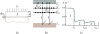
\includegraphics[scale=1.1]{figures/ch_06/fig_6_18.pdf}
		\caption[]{Generation of free charge carriers by light (internal photoeffect): (a)---absorption of light by a semiconducting specimen; (b)---excitation of free charge carriers from valence band, $1$ (intrinsic absorption), and from impurity levels, $2$ and $3$ (impurity absorption); (c)---dependence of absorption coefficient on wavelength ($1$---intrinsic absorption band, $2$ and $3$---impurity absorption bands, $\lambda_0$---threshold of photoeffect, $\ab{\lambda}{im$1$}$ and $\ab{\lambda}{im$2$}$---thresholds of impurity photoconductivity).}
		\label{fig:6_18}
	\end{center}
	\vspace{-0.7cm}
\end{figure}

To excite electrons from the levels of impurity atoms the photon energy should be $h\nu\geqslant\ab{E}{im}$, where $\ab{E}{im}$ is the ionization energy of those atoms. Such impurity levels in \fig{6_18}(b) are $E_1$ and $E_2$; the process of electron excitation from these levels is shown by arrows $2$ and $3$.

Thus, if
\begin{equation}\label{eq:6_44}
	\begin{split}
		h\nu\geqslant\ab{E}{g}\,\, &\text{in case of intrinsic semiconductors and}\\
		h\nu\geqslant\ab{E}{im}\,\, &\text{in case of impurity semiconductors,}
	\end{split}
\end{equation}

\noindent
then, excess charge carriers are generated in the semiconductor and its conductivity increases.

The process of internal liberation of electrons due to the action of light is termed the \textit{internal photoeffect}. The additional conductivity of a semiconductor irradiated with light is termed \textit{photoconductivity}. The name for initial conductivity due to the thermal carrier excitation is termed \textit{dark conductivity}, for it is the conductivity of the semiconductor kept in darkness. Light can excite excess carriers both, from the intrinsic and from the impurity levels, and accordingly, two types of conductivity can be distinguished: the \textit{intrinsic} and the \textit{impurity}. Using \eqn{6_44}, we can find the threshold of this process, that is, the maximum wavelength of light that is still photoelectrically active:
\begin{equation}\label{eq:6_45}
	\begin{split}
		\lambda_0 = \frac{ch}{\ab{E}{g}}\,\, &\text{for the intrinsic semiconductors and}\\
		\ab{\lambda}{im} = \frac{ch}{\ab{E}{im}}\,\, &\text{for impurity semiconductors,}
	\end{split}
\end{equation}

\noindent
where $c$ is the velocity of light.

The ionization energy for photoconductivity in pure semiconductors $\ab{E}{g}$ lies in the range of \SIrange{0.1}{5}{\electronvolt}, the majority having $\ab{E}{g}\approx$ \SIrange{1}{3}{\electronvolt}. The threshold for the latter lies in the visible part of the spectrum. Many impurity semiconductors have $\ab{E}{im}$ of the order of decimal fractions of an electron volt and even lower. For them the threshold lies in the infrared part of the spectrum.

Figure \ref{fig:6_18}(c) shows a schematic dependence of the absorption coefficient $k$ on the wavelength $\lambda$ for a semiconductor with two impurity levels $E_1$ and $E_2$ [\fig{6_18}(b)]. The absorption spectrum of such a semiconductor consists of three absorption bands: the intrinsic absorption band $1$ corresponding to the electron transition from the valence to the conduction band, and two impurity bands ($2$ and $3$). They correspond to electron transitions from the impurity levels $E_1$ and $E_2$ to the conduction band [\fig{6_18}(b)]. Light with $\lambda<\lambda_0=hc/\ab{E}{g}$ is practically completely absorbed near the surface
in a layer $x\approx\SI{e-6}{\metre}$ thick; its absorption coefficient is $k\approx\SI{e6}{\per\metre}$. The impurity absorption coefficient depends on the concentration of impurities but seldom exceeds $k\approx\SI{e3}{\per\metre}$. The less the impurity ionization energy $\ab{E}{g}$ the greater the maximum wavelength of photoconductivity is according to \eqn{6_45}.

The impurity photoeffect is only possible if the impurity levels $E_1$ and $E_2$ are occupied by electrons, that is, if the semiconductor's temperature is below the temperature of impurity exhaustion, $\ab{T}{s}$. For this reason, one usually has to cool the semiconductor to be able to observe photoconductivity, the necessary cooling temperatures being the lower the greater the maximum wavelength. For instance, gold-doped germanium has $\ab{\lambda}{im}=\SI{9}{\micro\metre}$ and must have liquid nitrogen cooling ($T=\SI{78}{\kelvin}$); germanium doped with the elements of Groups III or V of the Mendeleev periodic table has $\ab{\lambda}{im}=\SI{100}{\micro\metre}$ and needs liquid helium cooling ($T=\SI{4.2}{\kelvin}$).

If the intensity of light entering the semiconductor is $J$, the amount of luminous energy (the number of photons) absorbed in a unit volume of the semiconductor per unit time will be $kJ$, and the rate of carrier generation will be
\begin{equation}\label{eq:6_46}
	g = J k \beta
\end{equation}

\noindent
where $\beta$ is the quantum yield, which shows the number of free carriers generated by an absorbed photon.

In the absence of recombination, the number of excess carriers would grow continuously with time. The effect of recombination, whose rate rises with the concentration of excess carriers, is to establish
a stationary state in the semiconductor when the generation rate is equal to the recombination rate [see \eqn{5_49}]:
\vspace{-10pt}
\begin{equation}\label{eq:6_47}
	g = R = \frac{\Delta{n}_0}{\tau}.
\end{equation}

\noindent
This state is characterized by a constant (stationary) excess carrier concentration $\Delta{n}_0$ equal to
\begin{equation}\label{eq:6_48}
	\Delta{n}_0 = g \ab{\tau}{n} = J k \beta \ab{\tau}{n}.
\end{equation}

\noindent
Since the excess carriers have practically the same mobility as the equilibrium carriers, the stationary (steady-state) photoconductivity will be
\begin{equation}\label{eq:6_49}
	\ab{\sigma}{ph$0$} = q \beta k J \ab{u}{n} \ab{\tau}{n}.
\end{equation}

It follows from \eqn{6_49} that the stationary photoconductivity of a semiconductor and, consequently, the photosensitivity of semiconductor radiation detectors is proportional to the excess carrier lifetime $\ab{\tau}{n}$. From this point of view, it is advantageous to use materials with the highest possible $\ab{\tau}{n}$. However, this may substantially increase the time lag of the photodetector.

Indeed, consider the pattern of photoconductivity decay after the light source had been turned off (\fig{6_19}). The recombination process reduces the number of excess carriers in compliance with the law [see \eqn{5_50}]
\begin{equation*}
	\Delta{n} = \Delta{n}_0\, e^{-t/\ab{\tau}{n}}.
\end{equation*}

\begin{figure}[t]
	\begin{center}
		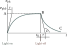
\includegraphics[scale=1]{figures/ch_06/fig_6_19.pdf}
		\caption[]{Rise in photoconductivity of a semiconductor illuminated by light and photoconductivity decay after illumination has ceased.}
		\label{fig:6_19}
	\end{center}
	\vspace{-0.7cm}
\end{figure}

The same will be true for the semiconductor's photoconductivity decay (curve BC):
\begin{equation}\label{eq:6_50}
	\ab{\sigma}{ph} = \ab{\sigma}{ph$0$}\, e^{-t/\ab{\tau}{n}}.
\end{equation}

It follows from \eqn{6_50} that the greater the excess carrier lifetime $\ab{\tau}{n}$ the slower the photoconductivity decay rate and, consequently, the greater will be the radiation detector's time lag.

It may easily be demonstrated that the tangent drawn to the photoconductivity decay curve $\ab{\sigma}{ph}(t)$ at point $t_0$ cuts off a section numerically, equal to $\ab{\tau}{n}$, the excess carrier lifetime. This method is often used for determining $\ab{\tau}{n}$.

Figure \ref{fig:6_19} also shows the pattern of the rise in photoconductivity after the semiconductor had been illuminated by a light pulse (curve $0$B). The photoconductivity rises gradually and reaches the ``plateau'' only after a lapse of some time. In this case too, a tangent to the curve $\ab{\sigma}{ph}(t)$ drawn at the origin cuts off a section of the straight line AB equal to $\ab{\tau}{n}$.

\textbf{Excitons.} In the act of photoconductivity the electrons from the valence band are transported to the conduction band and become free electrons. However, the process may take another course when the excited electron does not tear its connections with its counterpart hole in the valence band but forms an integral system with it. Ya. I. Frenkel proposed the term \textit{exciton} for such a system. The exciton is similar to an excited hydrogen atom---in both cases there is an electron moving about a unit positive charge and the energy spectrum is a discrete one (\fig{6_20}). The exciton levels are near the bottom of the conduction band. Since the excitons are electrically neutral, their appearance does not result in the generation of additional charge carriers. Because of that, the absorption of light is not accompanied by photoconductivity. The present point of view is that,
the formation of excitons can in some cases result in photoconductivity. The generated excitons for some time wander through the crystal. Colliding with phonons, impurity centres, or other lattice imperfections, the excitons may either recombine or ``decompose''. In the first case, the ground state is restored, the excitation energy being transmitted to the lattice or emitted in the form of light quanta
(luminescence). In the second case, a pair of free carriers, an electron and a hole, is created. They are responsible for the photoconductivity.

\begin{figure}[t]
	\begin{center}
		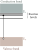
\includegraphics[scale=1]{figures/ch_06/fig_6_20.pdf}
		\caption[]{Exciton states in a semiconductor.}
		\label{fig:6_20}
	\end{center}
	\vspace{-0.7cm}
\end{figure}

Temperature greatly affects the photoconductivity of semiconductors. As the temperature decreases the number of dark carriers drops. The result is, firstly, an increase in the ratio of photoconductivity to the total conductivity and, secondly, an absolute increase in photoconductivity due to the decrease in the photocarrier recombination rate brought about by the decrease in the dark carrier concentration (the latter effect is observed only in semiconductors with prevailing direct recombination).

\textbf{Photoresistors.} The photoconductivity effect in some semiconductors is wide-ly utilized in photoresistors. Figure \ref{fig:6_21} shows schematically one of the types of photoresistors. It consists of a thin semiconducting film $2$ deposited on an insulating substrate $1$, of metal electrodes $3$, by means of which the photoresistor is connected into a circuit, and of a protective organic film $4$. The most sensitive photoresistors
are made of cadmium sulfide (CdS), the photoconductivity of which is \num{e5}-\num{e6} times higher than the dark conductivity. Also, in wide use are photoresistors made of lead sulfide (PbS), which are sensitive to the far infrared radiation. Other semiconducting materials are also being used.

The main advantage of the photoresistors over the vacuum photocells is their high light sensitivity. For instance, the sensitivity of selenium-cadmium photoresistors is \num{e5} times higher than that of
vacuum photocells. A disadvantage of the photoresistors is their time lag.

\begin{figure}[t]
	\begin{center}
		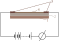
\includegraphics[scale=1]{figures/ch_06/fig_6_21.pdf}
		\caption[]{Schematic representation of a photoresistor: $1$---insulating substrate, $2$---semiconducting film, $3$---metal electrodes, $4$---protective coating.}
		\label{fig:6_21}
	\end{center}
	\vspace{-0.7cm}
\end{figure}

\textbf{Electrophotography.} The internal photoeffect in semiconductors is widely used in so-called \textit{electrophotography} or \textit{xerography}. The essence of this process is as follows. A thin film of high resistivity semiconductor (usually ZnO) is deposited on a sheet of paper. Before the photographic process the film is negatively charged by a gas discharge. When an image to be photographed is projected onto such paper, the surface charge from the illuminated parts leaks through the film much more readily than from the nonilluminated parts and accordingly an electric image of the object remains on paper after the exposition. To develop the electrical image the paper is sprayed by a weak spray of special dry paint, or ``toner''. The particles of toner are deposited on the negatively charged parts of the paper thus developing the image.

The image is fixed by heating the paper to the temperature at which the toner particles melt and adhere firmly to the paper. The main advantage of electrophotography over normal photography is the exclusion of chemical development and fixation processes. This makes it possible to increase the speed of the photographic process drastically, reducing the necessary time down to about ten seconds. However, as yet electrography is inferior to normal photography in accuracy and fineness of reproduction and, because of that, its application is limited to cases when great accuracy is not needed (for instance, for multiplying printed texts, cards, etc.). The well known Soviet-made duplicator ``Era'' operates on this principle.

\textbf{Semiconductor counters.} Apart from light, the internal photoeffect can be excited by irradiating the semiconductor with particles---with electrons, ions, \ce{\alpha}-particles, etc. Such particles passing through the semiconductor, generate free charge carriers and thus increase its conductivity or the current in a closed constant-voltage circuit. Since the number of generated carriers is proportional to the number of particles which enter the semiconductor, that number can be determined from the changes in the current. This fact enables semiconductor counters to be devised. Such counters are usually graduated not in units of current but directly in the number of particles. To enhance the sensitivity of the counter the variations of current flowing through the semiconductor are amplified with the aid of special electronic devices.

Semiconductor counters are now in a state of high perfection. They are widely used in nuclear research, in space technology, in medicine, in dosimetry, etc. They will probably play the leading role in radiation detection and spectrometry.

\section{Luminescence}\label{sec:61}

A heated body radiates energy the power and the spectral composition of which depend on the temperature of the body. This radiation is termed \textit{thermal}. Its main feature is that it is an equilibrium process. If we place a heated body into a cavity with walls of ideal reflectivity, a dynamical equilibrium is established between the atoms radiating energy and the radiation filling the cavity such that the number of atoms radiating energy and returning to the nonexcited state per unit time would be equal to the number of atoms absorbing radiation and going over to the excited state. This equilibrium can be maintained any length of time. Practically the same equilibrium radiation will be radiated by a heated body which is not surrounded by reflecting walls of a cavity if its temperature is held constant at the expense of energy supplied to it.

Bodies can be made to emit light not only by means of heating. Some materials emit light after they have been irradiated with visible or ultraviolet light, with X-rays, \ce{\gamma}-rays, electrons, or other particles, when placed in an electric field, etc. The emitted light may be in the visible part of the spectrum, although the temperature of the emitting body is low (room temperature and below). Such cold emission of light is termed \textit{luminescence} and the bodies exhibiting it
are termed \textit{luminophors}; the luminescence excited by light is termed \textit{photoluminescence}. In contrast to thermal radiation, luminescent radiation is a nonequilibrium process. Should a luminescent body be placed in a cavity with reflecting walls, it would loose energy by radiation because the radiated energy reflected by the walls would be absorbed by the body and entirely transformed into the energy of thermal vibrations of its atoms. Therefore, luminescence would eventually cease and the entire energy accumulated in the excited luminophor would be transformed into heat.

\begin{figure}[!t]
	\begin{minipage}[t]{0.48\linewidth}
		\begin{center}
			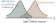
\includegraphics[scale=1]{figures/ch_06/fig_6_22.pdf}
			\caption[]{Illustration of Stoke's law.}
			\label{fig:6_22}
		\end{center}
	\end{minipage}
	\hfill{ }%\hspace{-0.1cm}
	\begin{minipage}[t]{0.48\linewidth}
		\begin{center}
			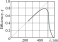
\includegraphics[scale=0.9]{figures/ch_06/fig_6_23.pdf}
			\caption[]{Illustration of Vavilov's law.}
			\label{fig:6_23}
		\end{center}
	\end{minipage}
\vspace{-0.3cm}
\end{figure}

The second important feature of luminescence is its long duration in comparison with the period of optic oscillations equal to \num{e-13}-\num{e-15} \si{\second}. The emission of light in the process of luminescence continues at least \SI{e-10}{\second} after the excitation has ceased. In some
instances the emission of light may continue for seconds, minutes, hours and even months after the excitation has ceased. In accordance with the duration of light emission, photoluminescence is divided into phosphorescence and fluorescence. Luminescence with a duration of under \SI{e-6}{\second} is usually termed \textit{fluorescence} and that with duration of over \SIrange{e-5}{e-6}\second{} is termed \textit{phosphorescence}.

The first quantitative investigation of luminescence was undertaken some 100 years ago by Sir George Gabriel Stokes. He succeeded in formulating the following rule which bears his name: the wavelength of light emitted in luminescence is longer than the wavelength of the absorbed light (\fig{6_22}). Subsequent experiments have proved that \textit{anti-Stokes} luminescence is also possible when the wavelength of luminescence is shorter than that of the excitation.

An important characteristic of luminescence is its efficiency $\eta$, first introduced by S. I. Vavilov. Efficiency is the ratio of the total energy emitted by a body in the process of luminescence to the energy absorbed by the body in the process of excitation. Figure \ref{fig:6_23} shows the dependence of $\eta$ on the wavelength of excitation. Inside some wavelength interval, the efficiency of luminescence rises in proportion to the wavelength but then drops drastically to zero. This rule was established by S. I. Vavilov and is known as Vavilov's law. The absolute value of the efficiency may be as high as $80\%$ or more.

Let us now discuss the mechanism of luminescence of solid crystals. Experiment shows that crystals with perfect lattice are practically incapable of luminescence. To make them exhibit luminescent properties defects should be created in their structure. The most effective defects are impurity atoms. Such impurities are termed \textit{activators}. Their contents in the matrix material hardly exceeds \num{e-4}. Materials widely used at present are the so-called \textit{phosphor crystals}---complex synthetic crystals with a defect structure possessing high luminescent properties. A phosphor crystal usually contains three components: the matrix, the activator and, the solvent. The materials frequently used as matrix materials are ZnS, CdS, CaS, etc.; as activators, the heavy metals Ag, Cu, Bi, Mn, etc., and as solvents, the low-melting salts. The spectral composition and the efficiency of luminescence depend both on the matrix material and the activator.

Figure \ref{fig:6_24} shows the energy band pattern of a fluorescent luminophor. There are impurity levels of the activator, A, between the filled band I and the vacant band II. When the activator atom absorbs a photon $h\nu$, an electron from the impurity level A is transported to the conduction band II. As a free electron it wanders freely in the
volume of the crystal until it meets an activator ion and recombines with it returning to the impurity level A. The recombination is accompanied by the emission of a quantum of fluorescent light. The decay time of luminescence of a luminophor is determined by the lifetime of the excited state of the activator atoms, which seldom exceeds \SI{e-9}{\second}. Therefore, fluorescence is a short-lived process and terminates almost immediately after the irradiation of the body has ceased.

\begin{figure}[!t]
	\begin{minipage}[t]{0.48\linewidth}
		\begin{center}
			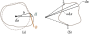
\includegraphics[scale=1.18]{figures/ch_06/fig_6_24.pdf}
			\caption[]{Energy diagram of fluorescent luminophor.}
			\label{fig:6_24}
		\end{center}
	\end{minipage}
	\hfill{ }%\hspace{-0.1cm}
	\begin{minipage}[t]{0.48\linewidth}
		\begin{center}
			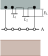
\includegraphics[scale=0.98]{figures/ch_06/fig_6_25.pdf}
			\caption[]{Diagram of electronic transitions in the act of phosphorescence.}
			\label{fig:6_25}
		\end{center}
	\end{minipage}
\vspace{-0.3cm}
\end{figure}

For durable luminescence characteristic of phosphorescence the luminophor must contain not only the activator atoms A but also electron traps $L$ near the bottom of the conduction band (\fig{6_25}). Such traps may be formed by impurity atoms, interstitial atoms, vacancies, etc. The light absorbed by the luminophor excited the activator atoms: the electrons from the impurity level A go over to the band II and become free electrons. Trapped by traps they loose their mobility together with the ability to recombine with the activator ions. To liberate an electron from the trap the energy $\ab{E}{L}$ should be expended. This energy the electron can obtain from the lattice vibrations. The time $\tau$ spent by the electron in a trapped state is proportional to $e^{\ab{E}{L}/(\ab{k}{B}T)}$; it may be quite large if $\ab{E}{L}$ is great enough.

The electron that left the trap wanders through the crystal until it is again trapped or recombines with an activator ion. In the latter case, a quantum of luminescent light is emitted. Hence, the traps serve as centres where the energy of absorbed photons is accumulated so as to be subsequently emitted in the form of luminescent light. The duration of this emission is determined by the time the electrons spend in the traps.

Experiments show that not in all cases is the transition of the electron from an excited state to the ground state accompanied by the emission of a light quantum. A much more frequent result is the generation of a phonon. For this reason, the purity of the phosphor crystals must satisfy the most severe requirements. Often a negligible impurity concentration (less than \num{e-4} percent) completely extinguishes the luminescence.

The quantum theory presents a simple explanation of the fundamental laws of luminescence including Stokes' and Vavilov's laws.

\textbf{Stokes' law.} When a luminophor is irradiated by light quanta, the energy of the quanta is partly spent on the excitation of the activator atoms and partly is transformed into energy of other types (mainly heat). Denote the fraction of the quantum's energy spent on exciting the activator atom by $\varepsilon$. When the atom returns from an excited to the ground state, a quantum of luminescent light will be emitted with its energy equal, evidently, to $\varepsilon$. The corresponding frequency is $\nu=\varepsilon/h$ and the wavelength is $\lambda=ch/\varepsilon$. Since the energy of the incident quantum $\varepsilon_0>\varepsilon$, the wavelength $\lambda$ of the luminescent light should be longer than that of the light which initiates luminescence ($\lambda>\lambda_0$) and this is what Stokes' law states.

When the incident quantum collides with an excited atom, its energy $\varepsilon_0=h\nu_0$ may be added to the excitation energy $\varepsilon$ causing the generation of a quantum with energy exceeding the energy of the one which initiates luminescence. This is the origin of \textit{anti-Stokes luminescence}.

\textbf{Vavilov's law.} Consider the simplest case of every incident photon $\varepsilon_0=h\nu_0$ generating a luminescent photon $\varepsilon=h\nu$ (quantum efficiency unity). Then, the efficiency of the luminescence will evidently be equal to the ratio of the energies of those photons: $\eta=\varepsilon/\varepsilon_0$. Since $\varepsilon=h\nu=hc/\lambda$, it follows that
\begin{equation}\label{eq:6_51}
	\eta = \frac{\nu}{\nu_0} = \frac{\lambda_0}{\lambda}.
\end{equation}

From \eqn{6_51}, we see that the luminescence efficiency should grow in proportion to the wavelength of the excitation, as required by Vavilov's law. When $\lambda_0$ attains a value for which the energy of the incident quanta is not enough to initiate luminescence, the efficiency drops abruptly to zero.

\section{Fundamentals of superconductivity}\label{sec:62}

\textbf{Phenomenon of superconductivity.} Investigating the role played by impurities in residual resistance, H. Kamerlingh Onnes in 1911 carried out experiments with ultrapure mercury. The results of those experiments were startling: at a temperature $\ab{T}{cr}=\SI{4.2}{\kelvin}$ the specific resistance $\rho$ of mercury fell to zero (\fig{6_26}). This phenomenon became known as \textit{superconductivity}. The temperature $\ab{T}{cr}$ at which the transition to the superconducting state takes place is termed \textit{critical}, or \textit{transition}, temperature. For thallium, tin and lead it is equal to \SI{2.53}{\kelvin}, \SI{3.73}{\kelvin} and \SI{7.19}{\kelvin}, respectively (\fig{6_26}).

Since according to Ohm's law $\rho=\mathcal{E}/i$, the condition $\rho=0$ means that, for a finite current density $i$, the intensity of the electric
field $\mathcal{E}$ at any point of the conductor is zero: $\mathcal{E}=0$.

Experiments carried out at M.I.T. showed that a current of several hundred amperes once induced in a superconducting ring continued to flow without attenuation for a whole year.

\begin{figure}[t]
	\begin{center}
		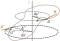
\includegraphics[scale=1.1]{figures/ch_06/fig_6_26.pdf}
		\caption[]{Abrupt change in specific resistance of mercury, tin, lead and thallium in the course of transition to superconducting state.}
		\label{fig:6_26}
	\end{center}
	\vspace{-0.7cm}
\end{figure}

Up to now over $20$ pure chemical elements and several hundred alloys and chemical compounds have been found to be superconductive. They have transition temperatures ranging from \SIrange{0.01}{20}{\kelvin}.

In 1933, W. Meissner and R. Ochsenfeld, found that the phenomenon of superconductivity consists not only in ideal conductivity, that is, zero specific resistance. The magnetic field is pushed out of the bulk of a superconductor no matter how this field was established---by an external magnet or by a current flowing in the superconductor itself. This means that the magnetic induction $\ab{B}{i}$ inside the superconductor is always zero as long as it is in the superconducting state.

In other words, the superconductor is an ideal diamagnetic whose magnetic susceptibility $\chi=-1$. It will be shown in the following chapter that normal diamagnetics have $|\chi|\ll 1$.

Hence, superconductivity is a combination of two simultaneous phenomena---that of ideal conductivity and of ideal diamagnetism.

The superconductive state can be destroyed by a magnetic field. The necessary magnetic field $\ab{H}{cr}$ is termed \textit{critical}. The value of $\ab{H}{cr}$ depends on the temperature: at $T=\ab{T}{cr}$, the critical field intensity is zero. With the decrease in temperature $\ab{H}{cr}$ rises and is maximal at absolute zero. The temperature dependence of $\ab{H}{cr}$ for lead and
tin is shown in \fig{6_27}.

\begin{figure}[t]
	\begin{center}
		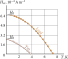
\includegraphics[scale=1]{figures/ch_06/fig_6_27.pdf}
		\caption[]{Temperature dependence of critical field intensity $\ab{H}{cr}$ in superconductor.}
		\label{fig:6_27}
	\end{center}
	\vspace{-0.7cm}
\end{figure}

\textbf{Fundamentals of theory of superconductivity.} Despite the fact that over $60$ years have gone by since superconductivity was first discovered, the microscopic theory of this phenomenon is a quite recent development due mainly to Bardeen, Cooper, Schrieffer. The abbreviation for it is the BCS theory. Let us discuss this theory in general terms.

\textbf{Gap in the energy spectrum of conduction electrons in a superconductor.} We again recall the causes of a finite electrical resistance of normal conductors, for instance, of metals in a normal state. If we neglect the periodic nature of the metal's lattice potential (the \textit{Sommerfeld model}), we can regard it as a potential trough for the electrons, having a flat bottom and filled by electrons up to the Fermi level $\ab{E}{F}$ (see \fig{3_4}). The kinetic energy of such electrons is given by \eqn{5_11}
\begin{equation*}
	E = \frac{p^2}{2m} = \frac{\hslash^2 k^2}{2m}.
\end{equation*}

Figure \ref{fig:6_28}(a) shows once again the $E$ versus $k$ dependence corresponding to \eqn{5_11}: thin horizontal lines denote the occupied levels, the solid line denotes the Fermi level $\ab{E}{F}$, and $\ab{k}{F}$ and---$\ab{k}{F}$ are wave vectors corresponding to this level.

The application of an electric field $\vec{\mathcal{E}}$ causes a change in the electron
distribution over the states [see \fig{6_1}(a)]; the electrons are transported from the left-hand side to the right-hand side. In \fig{6_28}(b), this corresponds to the transition of the electrons from the region of negative $k$'s to the region of positive $k$'s. Such transitions are possible since there is a practically unlimited number of unoccupied states above the Fermi level which the electrons can occupy.

\begin{figure}[t]
	\begin{center}
		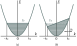
\includegraphics[scale=1]{figures/ch_06/fig_6_28.pdf}
		\caption[]{Dependence of free electron energy in conduction band of a metal on wave vector: (a)---in the absence of external field; (b)---external field $\vec{\mathcal{E}}$ imparts additional momentum to electrons, increasing their wave vector by $\Delta{k}$.}
		\label{fig:6_28}
	\end{center}
	\vspace{-0.7cm}
\end{figure}

Should there be no limiting factors, the momentum of the conduction electron would in time $\Delta{t}$ grow\footnote{The product $q\vec{\mathcal{E}}=\vec{F}$ is the force with which field $\vec{\mathcal{E}}$ acts on the electron. If $\Delta{t}$ is a time interval, $\vec{F}\Delta{t}$ is the impulse of force.} under the influence of the field $\mathcal{E}$ by an amount $p_{\mathcal{E}}=\hslash\Delta{k}=q\mathcal{E}\Delta{t}$, and a current of a density $i=qnvp_{\mathcal{E}}=qn/(q\mathcal{E}/m)\Delta{t}=(q^2n/m)\mathcal{E}\Delta{t}$ would be established in the conductor, its magnitude growing infinitely with time.
This would correspond to infinite specific conductance of the conductor, since
\begin{equation}\label{eq:6_52}
	\lim_{\Delta{t}\to\infty} \sigma = \lim_{\Delta{t}\to\infty} \frac{q^2 n}{m} \Delta{t} \to \infty.
\end{equation}

However, should it even be possible to realize condition \eqref{eq:6_52}, this would still not amount to ideal conductivity, which is characterized, as we have seen, by the condition that the current density for $\mathcal{E}=0$ is finite: $i\neq 0$. But the condition \eqref{eq:6_52} cannot be realized in any case. The factors that prevent this are the processes of electron scattering by lattice defects and, primarily, by thermal lattice vibrations---phonons---which are present down to absolute zero. Here, the main part is played by elastic scattering processes which change the electron's momentum to one directly opposite, so that they move over from the right-hand side of the distribution curve to the left-hand side. The corresponding transitions in \fig{6_28}(b) are those from the region of positive $k$'s to the region of negative $k$'s. The rate of the scattering processes is the greater the greater the field disturbs the equilibrium distribution of the electrons over the states, that is, the greater the displacement to the right of the distribution curve shown in \fig{6_1}(a) by a dotted line. Those processes bring the electron drift velocity down to the value $\ab{v}{d}=q\mathcal{E}\ab{\tau}{F}/m$, the current density to $i=q^2n\mathcal{E}\ab{\tau}{F}/m$, and the specific conductance to $\sigma=q^2n\ab{\tau}{F}/m$, where $\ab{\tau}{F}$ is the relaxation time of the electrons occupying levels close to the Fermi level.

Let us make the following point important for the future. At least two conditions should be fulfilled to make elastic transitions, which are responsible for finite electrical resistance of a normal metal, possible: (a) there should be states the scattered electrons can occupy (in other words, the corresponding energy levels should lie in the allowed energy band); (b) the states the scattered electrons are to occupy must not already be occupied.

For a normal metal with an energy spectrum of conduction electrons as shown in \fig{6_28}, both those conditions are fulfilled making the scattering processes possible.

Can a model of the energy spectrum of conduction electrons be built which would make scattering processes (at least under certain conditions) impossible even in the presence of scattering centres---phonons, impurity atoms, etc.?

Apparently, yes. Such a spectrum is shown in \fig{6_29}(a). The difference between it and the spectrum shown in \fig{6_28} is that in it there is an energy gap $\ab{E}{e.g}$ with the Fermi level $\ab{E}{F}$ in the middle. The lower part of the conduction band is completely occupied by electrons; the upper part above the gap is completely free. The band pattern looks like that of an intrinsic semiconductor at $T=\SI{0}{\kelvin}$ whose specific conductance in case of such occupation of the bands is zero. Since the metal retains its high specific conductance at $T\approx\SI{0}{\kelvin}$, it should be presumed that in contrast to a semiconductor whose energy gap (the forbidden band) does not change its position in an external field, the $\ab{E}{e.g}$ in the conduction band of the metal moves in the electric field together with the electron distribution, as shown in \fig{6_29}(b). During a finite time interval $\Delta{t}$, the field $\mathcal{E}$ exists in the superconductor, the electron's wave vector increases by an amount $\Delta{k}=p_{\mathcal{E}}/\hslash=q\mathcal{E}\Delta{t}/\hslash$ and the energy gap $\ab{E}{e.g}$ shifts to the right together with the electron distribution by a distance $\Delta{k}$.

\begin{figure}[t]
	\begin{center}
		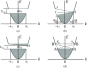
\includegraphics[scale=1.05]{figures/ch_06/fig_6_29.pdf}
		\caption[]{Energy spectrum of conduction electrons in metal with a mobile energy gap (explanation in text).}
		\label{fig:6_29}
	\end{center}
	\vspace{-0.7cm}
\end{figure}

Now let us consider the possibility for the electron $q$ occupying the upper level of the right-hand subband to be scattered. The arrows $1$, $2$, $3$ in \fig{6_29}(b) show the possible scattering processes: $1$ is elastic scattering resulting in the change from $k$ to $-k$; $2$ are transitions to the levels of the lower left-hand subband; $3$ are transitions to the levels of the upper left-hand subband. It may easily be seen that transitions $1$ are forbidden since they terminate in the forbidden
part of the energy spectrum, namely $\ab{E}{e.g}$. Transitions $2$ are forbidden by the Pauli exclusion principle, since the corresponding levels
are already occupied by electrons. Transitions $3$, although allowed, require an ionization energy equal to $\ab{E}{e.g}$. If the metal's temperature
is low enough so that the mean phonon energy $\hslash\ab{\omega}{ph}<\ab{E}{e.g}$, those transitions are impossible\footnote{To be exact, there are phonons with an energy $\hslash\ab{\omega}{ph}>\ab{E}{e.g}$ capable of
exciting electrons from the lower subband to the states of the upper subband even at the lowest temperature. This should cause the appearance of vacant levels in the lower subband and of ``normal'' electrons in the upper subband. One would think that the appearance of vacant levels in the lower subband would bring about the scattering of electrons responsible for ideal conductivity; in other words, that it would in effect destroy superconductivity. Actually, as a more detailed consideration shows, a rise in temperature is accompanied by a narrowing of the energy gap [\fig{6_29}(c)] so that no vacant level capable of scattering the electrons of the lower subband remains in it. In other words, phonons with an energy $\hslash\ab{\omega}{ph}>\ab{E}{e.g}$ not only transform a superconducting electron A into a normal one B$'$ but destroy the superconducting state of this electron and of the electron A$'$, which was paired with A, by exciting it to the
normal state [\fig{6_29}(d)]. As temperature rises the number of ``energetic'' phonons decreases, the width of the energy gap decreases together with the
number of superconducting electrons. On the contrary, the number of normal electrons rises. At $T=\ab{T}{cr}$, the width of the gap vanishes (\fig{6_34}), all electrons go over to the normal state, and superconductivity is destroyed.}.

Hence, there are conditions in which even in the presence of such scattering centres as phonons, the scattering processes limiting the conductivity in a metal, whose electron energy spectrum has a ``mobile gap'' (\fig{6_29}), cannot take place. Accordingly, such a metal may become an ideal conductor, just like a superconductor.

Let us look again at \fig{6_29}(a). The tangent to the curve $E(k)$ near the top of the lower, filled, part of the conduction band runs horizontally ($\diffin{E}{k}=0$) and, accordingly, the translational velocity of the electrons occupying these levels $v=\hslash^{-1}(\diffin{E}{k})=0$, although their momentum $p_1$ and wave vector $k_1=p_1/\hslash$ are quite large. We encountered a similar model when we discussed semiconductors (see \fig{5_12}); this property of the electrons will prove to be essential in constructing the model of superconductivity.

Figure \ref{fig:6_30}(a) shows the dependence of the density of states in the conduction band of a normal metal on energy for $T=\SI{0}{\kelvin}$ and \fig{6_30}(b) the pattern of this dependence in the presence of a gap $\ab{E}{e.g}$ in the conduction band. Near the edges of the gap the density of the states is higher and because of that the band made shorter by $\ab{E}{e.g}/2$ still has enough states to accept all the electrons of the conduction band.

\begin{figure}[t]
	\begin{center}
		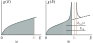
\includegraphics[scale=1.05]{figures/ch_06/fig_6_30.pdf}
		\caption[]{Variation of density of states of free electrons in metal with the appearance of an energy gap in the conduction band: (a)---density of states versus energy plot for a normal metal; (b)---ditto for a metal with a gap in its conduction band.}
		\label{fig:6_30}
	\end{center}
	\vspace{-0.7cm}
\end{figure}

Hence, if we were to prove that metals can actually have an electron energy spectrum with a ``gap'' and if the causes of its appearance could be established, the miracle of the ideal conductivity of superconductors would generally be unveiled. For this reason, the efforts of investigators in superconductivity were concentrated on the experimental verification of the presence of such a gap in the energy spectrum of superconducting metals.

At present, a number of methods have been devised capable not only of detecting the gap but also of measuring its width. One of them is based on the study of far infrared radiation absorption by metals. The idea of the method is as follows. Should a superconductor be irradiated with electromagnetic radiation of continuously varying frequency $\omega$, it would not be absorbed as long as the energy of its quantum remained less than the width of the gap $\ab{E}{e.g}$ (of course,
if there is such a gap). Intense absorption should start at a frequency $\ab{\omega}{cr}$, for which $\hslash\ab{\omega}{cr}=\ab{E}{e.g}$, increasing with the frequency to values common to a normal metal. Measuring $\ab{\omega}{cr}$ one can determine $\ab{E}{e.g}$.

The experiments convincingly proved that there is a gap in the electron energy spectrum of superconductors. Table \ref{table:6_6} shows the
values of the gap width at $T=\SI{0}{\kelvin}$ for some metals together with the transition temperature. We see that the gap $\ab{E}{e.g}$ is very narrow, approximately \SIrange{e-3}{e-2}{\electronvolt} wide, and that there is a direct connection between the gap's width and the transition temperature $\ab{T}{cr}$; the higher the $\ab{T}{cr}$ the greater the $\ab{E}{e.g}$ is.

\begin{table}[!b]
	\renewcommand{\arraystretch}{1.2}
	\caption{}
	\vspace{-0.6cm}
	\label{table:6_6}
	\begin{center}\resizebox{0.8\linewidth}{!}{
			\begin{tabular}{lcccccc}
				\toprule[1pt]
                & Al & Sn & Hg & V & Pb & Nb\\
                \midrule[0.5pt]\midrule[0.5pt]
                $\ab{E}{e.g}(0)$ (\SI{e3}{\electronvolt}) & $3.26$ & $11.0$ & $16.4$ & $14.3$ & $21.4$ & $22.4$\\
				$\ab{T}{cr}$ (\si{\kelvin}) & $1.2$ & $3.73$ & $4.15$ & $4.9$ & $7.19$ & $9.22$\\
				$\ab{E}{e.g} = 3.5\ab{k}{B}\ab{T}{cr}$ (\SI{e3}{\electronvolt}) & $3.6$ & $11.2$ & $12.5$ & $14.8$ & $21.7$ & $27.7$\\
				\bottomrule[1pt]
			\end{tabular}
	}\end{center}
\end{table}

After the presence of a gap in the energy spectrum of conduction electrons in superconductors was proved experimentally, attention turned to the problem of the origin of this gap.

\textbf{Electron pair formation.} As we already know, the formation of forbidden bands in the energy spectrum of semiconductors is due to the interaction of the electrons with the periodic field of the crystal lattice.

It would be natural to suppose that the energy gap in the conduction band of a metal in the superconducting state is also due to some additional electronic interaction that appears when the metal enters that state. Its origin is as follows.

\begin{figure}[t]
	\begin{center}
		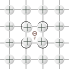
\includegraphics[scale=1.0]{figures/ch_06/fig_6_31.pdf}
		\caption[]{Moving electron polarizes the lattice and pulls positive ions a little away from their equilibrium sites, thereby creating an excess positive charge which attracts another electron so that it forms an electron pair with the first electron.}
		\label{fig:6_31}
	\end{center}
	\vspace{-0.7cm}
\end{figure}

A free electron moving through the lattice interacts with the ions, ``pulling'' them from their equilibrium sites (\fig{6_31}) and creating an excess positive charge that may attract another electron. For this reason, apart from the usual Coulomb repulsion, a force of attraction can arise between the electrons owing to the presence of the
positive ion lattice. If this force of attraction exceeds the force of repulsion, it will be advantageous from the viewpoint of energy for
the electrons to associate into couples. These became known as \textit{Cooper pairs}.

The formation of a Cooper pair results in the reduction in the energy of the two electrons by the amount equal to the binding energy of the electrons in the pair, $\ab{E}{b}$. This means that a conduction electron, which in a normal metal had a maximum energy $\ab{E}{F}$ at $T=\SI{0}{\kelvin}$ [see \fig{6_28}(a)], in the superconducting state has an energy $\ab{E}{b}/2$ less (the energy per pair being $\ab{E}{b}$ less) since this is the energy that must be spent to break up the pair and move the electrons to the normal state. Therefore, in the one-electron spectrum there must be a gap of $\ab{E}{e.g}=2\ab{E}{b}$ between the upper level of a coupled electron and the lower level corresponding to the normal state, which is required
for superconductivity. It may easily be seen that this gap is mobile, that is, it can shift in an external field together with the electron distribution curve over the states.

Figure \ref{fig:6_32} is a schematic representation of a Cooper pair. It consists of two electrons oscillating about the induced positive charge, which in some ways resembles a helium atom. Each electron of the pair may have a large momentum $\ab{p}{F}$ and a large wave vector $\ab{k}{F}$; the pair as a whole (its centre of masses), on the other hand, can remain stationary having zero translational velocity. This explains a paradoxical property of the electrons occupying the upper levels of the filled part of the conduction band in the presence of a gap [see \fig{6_29}(a)]. Such electrons have very large $p$'s and $k$'s ($p\approx\ab{p}{F}$ and $k\approx\ab{k}{F}$) and a translational velocity $v\propto\diffin{E}{k}=0$. Since the central positive charge is induced by the moving electrons themselves, the Cooper pair acted upon by an external field can freely drift in the crystal, the energy gap moving with the electron distribution, as shown in \fig{6_29}(b). Hence, the conditions for superconductivity are fulfilled from this point of view as well.

\begin{figure}[!t]
	\begin{minipage}[t]{0.48\linewidth}
		\begin{center}
			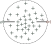
\includegraphics[scale=1]{figures/ch_06/fig_6_32.pdf}
			\caption[]{Schematic model of a Cooper pair.}
			\label{fig:6_32}
		\end{center}
	\end{minipage}
	\hfill{ }%\hspace{-0.1cm}
	\begin{minipage}[t]{0.48\linewidth}
		\begin{center}
			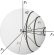
\includegraphics[scale=1]{figures/ch_06/fig_6_33.pdf}
			\caption[]{Estimating the number of electrons capable of forming Cooper pairs.}
			\label{fig:6_33}
		\end{center}
	\end{minipage}
\vspace{-0.3cm}
\end{figure}

However, not all the conduction electrons can form Cooper pairs. Since this process involves a change in energy, only electrons that can change their energy can form pairs. Only the electrons in a narrow strip close to the Fermi level (the Fermi electrons) are free from this limitation. A rough estimate gives the fraction of such electrons as being approximately \num{e-4} of the total number of electrons and the width of the strip of the order of $\num{e-4}\ab{p}{F}$.

Figure \ref{fig:6_33} shows a Fermi sphere of a radius $\ab{p}{F}$ in momentum space. Rings $\deriv{l}$ wide make angles $\varphi_1$, $\varphi_2$, $\varphi_3$ with the $p_y$ axis. The electrons the ends of whose momentum vectors $\ab{\vec{p}}{F}$ lie within the area of a given ring, make up a group every member of which has the same absolute value of momentum $\ab{p}{F}$. The number of electrons in each group is proportional to the area of the respective ring. Since the area of the ring rises with $\varphi$ so does the number of electrons in the band. Electrons of any group may form pairs, but the maximum number of pairs will be formed by the electrons of the more numerous group. The latter is made up of electrons whose momenta are equal in magnitude and opposite in direction.
The ends of the vectors $\ab{\vec{p}}{F}$ of such electrons are not limited to a narrow band but spread over the entire Fermi surface. Those electrons are so numerous in comparison with any other electrons that practically only one group of Cooper pairs is formed---that made up of electrons whose momenta are equal in magnitude and opposite in direction.

A remarkable peculiarity of such pairs is the ordering of their momenta: the centres of masses of all the pairs have identical momenta, being zero when the pairs are at rest and nonzero when the pairs move in the crystal. The result is a rather rigid correlation between the motion of every single electron and the motion of all the other electrons bound into pairs.

The electrons ``move like mountain-climbers tied together by a rope: should one of them leave the ranks due to the irregularities of the terrain (caused by the thermal vibrations of the lattice atoms) his neighbours would pull him back''\footnote{Ya. I. Frenkel: \textit{Introduction to the Theory of Metals}, GITTL, Moscow (1950) (in Russian).}. This property makes the ensemble of Cooper pairs little susceptible to scattering. Accordingly, should the pairs acted upon by some external force be set in motion, the current established by them would continue to flow in the superconductor indefinitely even after the factor that brought it to life ceased to operate. Since only the electric field $\mathcal{E}$ can play the role of such a factor, this means that in a metal, in which Fermi electrons are bonded into Cooper pairs, a once excited electric current $i$ can remain unaltered even after the field has vanished: $i = $ constant at $\mathcal{E}=0$. This proves that the metal is actually in the superconducting state and that its conductivity is ideal. Such state of the electrons may be roughly compared with the state of a body moving without friction: the body having received a momentum can move indefinitely and its momentum remains constant.

In the above, we compared a Cooper pair to a helium atom. However, such a comparison should be treated very cautiously. As was already stated, the positive charge is not exactly constant and stationary, as in the case of a helium atom, but is induced by the moving electrons themselves and moves with them. Moreover, the binding energy of the electrons in a pair is many orders of magnitude less than their binding energy in the helium atom. According to \tab{6_6} the binding energy of Cooper pairs $\ab{E}{b}=$ \SIrange{e-3}{e-2}{\electronvolt}, the corresponding value for the helium atom being  $\ab{E}{b}=\SI{24.6}{\electronvolt}$. Because
of that, the dimensions of the Cooper pair are many orders of magnitude larger than that of the helium atom. Calculations show the effective diameter of a pair to be $L\approx$ \SIrange{e-7}{e-6}{\metre}; another term for it is \textit{coherence length}. There are about \num{e6} centres of masses of Cooper pairs inside the effective volume $L^3$ of one such pair. For this reason, such pairs cannot be regarded as separately existing ``quasimolecules''. On the other hand, the accompanying colossal overlapping of the wave functions of numerous pairs enhances the electron pairing effect so that it manifests itself in macroscopic proportions\footnote{There is another analogy, a very profound one at that, between a Cooper pair and a helium atom. The essence of it is that an electron pair constitutes a system with integral spin, the same as the helium atom \ce{^4_2He} does. It is a known fact that the superfluidity of helium may be considered as the result of a peculiar effect of bosons condensing on the lowest energy level. From this point of view,
superconductivity may be regarded as superfluidity of the Cooper electron pairs. The analogy is a still more far-reaching one. Another helium isotope \ce{^3_2He}, whose nucleus has a half-integral spin, does not exhibit superfluidity. But a most striking new discovery is that in the lowest temperature range the atoms of \ce{^3_2He} can form pairs quite like the Cooper pairs and the liquid becomes superfluid. One is justified in saying that the superfluidity of \ce{^3_2He} is a sort of superconductivity of its atomic pairs.}.

Hence, electron pairing is a typical collective effect. There are no forces of attraction acting between two isolated electrons to make their coupling possible. In effect, the entire ensemble of the Fermi electrons together with the lattice atoms takes part in the formation of a pair. Because of that, the binding energy (the gap width $\ab{E}{e.g}$) too depends on the state of the electron-atom ensemble as a whole. At absolute zero, when all the Fermi electrons are in pairs, the width of the gap is at its maximum, $\ab{E}{e.g}(0)$. The rise in temperature is accompanied by the generation of phonons capable in the act of scattering of transmitting energy to the electrons sufficient to break up the pair. At low temperatures the concentration of such phonons
is not large and the breaking up of a pair is a rare event. The disappearance of some pairs cannot, naturally, lead to the disappearance of the gap for the remaining pairs but makes it somewhat narrower,
with the edges of the gap drawing closer to the Fermi level [see \fig{6_29}(c)]. With a further rise in temperature the phonon concentration grows very rapidly, their mean energy growing as well. The result is a steep rise in the bear-up rate of the pairs and, accordingly, a drastic decrease in the gap width for the remaining pairs. At some temperature $\ab{T}{cr}$ the gap disappears altogether (\fig{6_34}), its edges merging with the Fermi level and the metal returning to the normal state. The temperature $\ab{T}{cr}$ is just the critical transition temperature that was mentioned at the beginning of the section.

\begin{figure}[t]
	\begin{center}
		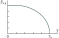
\includegraphics[scale=1.0]{figures/ch_06/fig_6_34.pdf}
		\caption[]{Variation of the energy gap $\ab{E}{e.g}(T)$.}
		\label{fig:6_34}
	\end{center}
	\vspace{-0.7cm}
\end{figure}

It follows then that the critical temperature for the transition of a metal to the superconductive state should be the greater the greater the gap width at absolute zero, $\ab{E}{e.g}(0)$, is. The BCS theory gives the following approximate dependence of $\ab{E}{e.g}(0)$ on $\ab{T}{cr}$:
\begin{equation}\label{eq:6_53}
	\ab{E}{e.g}(0) = 3.5 \ab{k}{B} \ab{T}{cr}
\end{equation}

which is in good agreement with experiment (see the last line in \tab{6_6}).

\textbf{Behaviour in an external electric field.} Connect a long cylindrical superconducting specimen into an electric circuit, as shown in \fig{6_35}(a). As the circuit is closed, a homogeneous electric field is established in the specimen, $\mathcal{E}=V/l$, where $V$ is the voltage across the specimen and $l$ is its length. Acted upon by the field $\mathcal{E}$ all Cooper pairs contained in the specimen will start to move against the field with the same acceleration
\begin{equation*}
	a = \frac{2 q \mathcal{E}(t)}{2m} = \frac{q\mathcal{E}(t)}{m}
\end{equation*}

\noindent
where $2q$ is the pair's charge, and $2m$ its mass.
The current density in the superconductor will start to grow:
\begin{equation*}
	\diff{i}{q} = 2q \parenthesis{\frac{\ab{n}{s}}{2}}\, \diff{\ab{v}{d}}{t} = q \ab{n}{s} a = \frac{q^2 \ab{n}{s}}{m} \mathcal{E}(t)
\end{equation*}

\noindent
where $\ab{v}{d}$ is the drift velocity of the pairs, $\ab{n}{s}/2$ their number, and $\ab{n}{s}$ is the concentration of ``superconducting'' electrons.

\begin{figure}[t]
	\begin{center}
		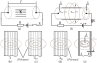
\includegraphics[scale=1.1]{figures/ch_06/fig_6_35.pdf}
		\caption[]{Behaviour of superconductor connected into an electric circuit (see text).}
		\label{fig:6_35}
	\end{center}
	\vspace{-0.7cm}
\end{figure}

The current $i$ generates a solenoidal magnetic field $H$ in the superconductor [\fig{6_35}(b)]. Since $i$ grows with time so does the magnetic field $H$. This results in the appearance of an induced electric field $\ab{\mathcal{E}}{in}$ in directed against $\mathcal{E}$ and of an induced current $\ab{i}{in}$ directed against $i$ [\fig{6_35}(c)]. The current $\ab{i}{in}$ generates a magnetic field $\ab{H}{in}$ directed against $H$ [\fig{6_35}(d)]. The result is the compensation
of the field $\mathcal{E}$ inside the superconductor by the field $\ab{\mathcal{E}}{in}$ and of the field $H$ by the field $\ab{H}{in}$, so that the resulting electric field in the specimen $\mathcal{E}=0$ [\fig{6_35}(f)] together with the resulting magnetic field $\ab{H}{int}=0$. For such compensation to continue it is necessary, firstly, that the current of Cooper pairs, $i$, be maintained
in the specimen indefinitely after the end of transient processes. To this end, the specimen's resistance should be zero and this is so if the specimen is in the superconducting state. Secondly, this current should be localized in a thin surface layer $\lambda$ of the superconductor [Figures \ref{fig:6_35}(e,f)], for in this case it does not generate a magnetic field inside the specimen but generates an external field $H$ in the surrounding space just as a normal current does.

Hence, after transient processes come to an end the following stationary state is established in the specimen:
\begin{equation*}
	\mathcal{E}=0,\quad i=\text{constant},\quad \ab{H}{int}=0.
\end{equation*}

\noindent
The first two conditions correspond to ideal conductivity and the third to ideal diamagnetism. In the stationary state, Cooper pairs move without acceleration (free motion) with the same drift velocity $\ab{v}{d}=p_{\mathcal{E}}/m$, where $p_{\mathcal{E}}$ is the momentum accumulated by the pair during the time the circuit was closed. The current set up by them is
\begin{equation*}
	i = 2q \parenthesis{\frac{\ab{n}{s}}{2}} \ab{v}{d} = q \ab{n}{s} \frac{p_{\mathcal{E}}}{m}.
\end{equation*}

\noindent
As has already been stated before, this current is localized in a thin surface layer $\lambda$ of the sample, the magnetic field of the current being concentrated in this layer [Figures \ref{fig:6_35}(e,f)]. The parameter $\lambda$ is
termed the \textit{penetration depth}. Theory gives the following expression for this parameter:
\begin{equation}\label{eq:6_54}
	\lambda = \parenthesis{\frac{m}{q^2 \ab{n}{s} \mu_0}}^{1/2}
\end{equation}

\noindent
where $\mu_0$ is the permeability of free space. For different superconductors $\lambda$ lies in the range from \SIrange{4e-8}{e-7}{\metre}.

It follows from \eqn{6_54} that at $T=\ab{T}{cr}$, when the concentration of ``superconducting'' electrons vanishes, $\lambda$ becomes infinite. Physically, this means that, as the metal returns to the normal state the layer $\lambda$ in which the magnetic field is localized spreads across the entire cross section of the sample and ideal diamagnetism vanishes.

\textbf{Behaviour of superconductor in magnetic field.} Now let us suppose that a magnetic field $\ab{H}{ext}$ is set up in space containing a cylindrical superconducting sample [\fig{6_36}(a)]. The field induces a solenoidal electric field in the sample which sets up a solenoidal electric current $\ab{i}{in}$. The current $\ab{i}{in}$ creates a magnetic field $\ab{H}{in}$ [\fig{6_36}(b)] directed against the external field and compensates it.
The field $\ab{H}{in}$ in its turn generates the current $\ab{i}{in}'$ which compensates the current $\ab{i}{in}$ [\fig{6_36}(c)]. The overall effect is the compensation of the external field $\ab{H}{ext}$ by the field $\ab{H}{in}$ and of the current $\ab{H}{in}$ by $\ab{H}{in}'$ [\fig{6_36}(d)].
The total induced current flows in a thin surface layer $\lambda$ in which its magnetic field that compensates the external field is localized. After the termination of transient processes the same steady state is established in the sample as was the case when an emf was applied to it:
\begin{equation*}
	\mathcal{E}=0,\quad i=\text{constant},\quad \ab{H}{int}=0.
\end{equation*}

\noindent
Naturally, this state can be established only if the current $\ab{i}{in}$ induced during the time the magnetic field was switched on continues indefinitely, that is, if the sample is in the superconducting state.

\begin{figure}[t]
	\begin{center}
		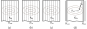
\includegraphics[scale=1.2]{figures/ch_06/fig_6_36.pdf}
		\caption[]{Behaviour of superconductor in magnetic field (explanation in text).}
		\label{fig:6_36}
	\end{center}
	\vspace{-0.7cm}
\end{figure}

\textbf{Destruction of superconducting state by fields.} Before the field is switched on, the momenta of the electrons making up a pair are equal in magnitude and opposite in direction, the momentum of the centre of masses of the pair is zero. Acted upon by the field $\mathcal{E}$ every pair as a whole attains some drift velocity $\ab{v}{d}$ and increases its energy by the amount
\begin{equation*}
	\Delta{E} = 2 \parenthesis{\frac{m\ab{v}{d}^2}{2}}.
\end{equation*}

If this energy exceeds the binding energy of the pair $\ab{E}{b}=\ab{E}{e.g}/2$, the pairs start to break up and the superconducting state would start to vanish. For this reason, the condition for the transition of a metal from the superconducting to the normal state may be written as follows:
\begin{equation*}
	2 \parenthesis{\frac{m\ab{v}{d}^2}{2}} \geqslant \frac{\ab{E}{e.g}}{2}.
\end{equation*}

\noindent
From here we can easily find the drift velocity
\begin{equation*}
	\ab{v}{d} = \parenthesis{\frac{\ab{E}{e.g}}{2m}}^{1/2}
\end{equation*}

\noindent
and the current density
\begin{equation}\label{eq:6_55}
	\ab{i}{cr} = q \ab{n}{s} \ab{v}{d} = q \ab{n}{s} \parenthesis{\frac{\ab{E}{e.g}}{2m}}^{1/2}
\end{equation}

\noindent
for the case when superconductivity in a metal begins to vanish. Setting $\ab{E}{e.g}=\SI{5e-4}{\electronvolt}$, $q=\SI{1.6e-19}{\coulomb}$, and $\ab{n}{s}=\SI{e-18}{\per\centi\metre\cubed}$, we obtain $\ab{v}{d}=\SI{1.8e4}{\metre\per\second}$ and $\ab{i}{cr}=\SI{2.5e5}{\ampere\per\centi\metre\squared}$.

With account taken of the fact that the current $i$ sets up a magnetic field on the surface of the sample of intensity
\begin{equation}\label{eq:6_56}
	H = i \lambda,
\end{equation}

\noindent
($\lambda$ is the penetration depth of the magnetic field into the superconductor) condition \eqref{eq:6_55} may be formulated as follows: the superconducting state of the sample will be destroyed when the intensity of the magnetic field on its surface will attain the following critical value:
\begin{equation}\label{eq:6_57}
	\ab{H}{cr} = \ab{i}{cr} \lambda.
\end{equation}

\noindent
Substituting $\lambda$ from \eqn{6_54} and $\ab{i}{cr}$ from \eqn{6_55} we obtain
\begin{equation}\label{eq:6_58}
	\ab{H}{cr} = \parenthesis{\ab{n}{s} \frac{\ab{E}{e.g}}{2 \mu_0}}^{1/2}.
\end{equation}

\noindent
For $\ab{E}{e.g}=\SI{5e-4}{\electronvolt}$ and $\ab{n}{s}=\SI{e18}{\centi\metre\cubed}$, $\ab{H}{cr}\approx\SI{e4}{\ampere\per\metre}$ (or $100$ Oe).

Thus, when the magnetic field on a superconductor's surface attains the critical value $\ab{H}{cr}$ determined by condition \eqref{eq:6_58}, the superconductivity is destroyed. Since the gap width substantially depends on temperature [see \eqn{6_53}], $\ab{i}{cr}$ and $\ab{H}{cr}$ should also depend on temperature, their values decreasing with the rise in temperature. The BCS theory gives the following dependence of $\ab{H}{cr}$ and $\ab{I}{cr}$ on absolute temperature:
\begin{align}
	\ab{H}{cr} &= \ab{H}{cr}(0) \bracket{1 - \parenthesis{\frac{T}{\ab{T}{cr}}}^2}, \label{eq:6_59}\\
	\ab{I}{cr} &= \pi d \ab{H}{cr},\quad \text{for}\quad d\gg\lambda, \label{eq:6_60}
\end{align}

\noindent
where $\ab{H}{cr}(0)$ is the critical magnetic field intensity at $T=\SI{0}{\kelvin}$, and $d$ is the diameter of the specimen. There is a satisfactory agreement between those relations and experiment.

\textbf{Practical uses of superconductivity.} The field of practical application of superconductivity widens from year to year. First, it serves as a basis for superconducting magnets. Such magnets are solenoids or electromagnets with a ferromagnetic core with the winding made of a superconducting material. Calculations show that to establish a magnetic field intensity of \SI{8e6}{\ampere\per\metre} ($\approx$ \num{e5} Oe) in a solenoid of a diameter of one metre, a superconducting magnet requires \num{e4} times less power than an ordinary electromagnet. Recently, superconducting magnets using \ce{Nb3Sn} have been fabricated which enable magnetic fields up to \SI{6e6}{\ampere\per\metre} ($\approx$ \num{7e4} Oe) to be produced.

Superconductivity is also being utilized to design modulators (converters of weak constant current into an audio-frequency current), rectifiers for the detection of modulated high frequency oscillations in which the use is made of the nonlinearity of the superconductor's resistance in the transitional region, commutators (noncontact switches utilizing the phenomenon of superconductivity), cryotrons (superconducting four-poles in which the magnetic field at the input controls the output resistance), persistors and persistrons (superconducting memory elements for memory devices), etc.

Of highest practical importance is the problem of high temperature superconductivity. Of all the known materials the highest transition temperature is that of the alloy \ce{(Nb3Al)4+Nb3Ge} whose $\ab{T}{cr}\approx\SI{20}{\kelvin}$. To obtain such a temperature liquid helium is needed. What are the prospects for developing materials with higher critical temperatures?

The BCS theory demonstrates that $\ab{T}{cr}$ is directly related to the force of attraction between the electrons in the superconductor and is determined from the following approximate expression:
\begin{equation}\label{eq:6_61}
	\ab{T}{cr} = \Theta\, e^{-1/g}
\end{equation}

\noindent
where $\Theta$ is the Debye temperature, and $g$ is a constant (not exceeding $1/2$ and usually less) dependent on the attraction force between the electrons. For $g=1/3$, the maximum critical temperature obtainable with a material with $\Theta=\SI{500}{\kelvin}$ would be $\ab{T}{cr}=\Theta\,e^{-3}=0.05\Theta=\SI{25}{\kelvin}$. Naturally, this estimate is a very rough one but still it makes it clear that it is impossible to obtain high temperature superconductivity ($\ab{T}{cr}>\SI{100}{\kelvin}$) with the electron pairing mechanism discussed above.

Simultaneously, with the development of superconducting materials with increased $\ab{T}{cr}$ utilizing the electron pairing effect via positively charged lattice ions, an intensive search for other mechanisms of electronic interaction capable of more efficient attraction and, consequently, of providing superconductive materials with substantially greater transition temperatures $\ab{T}{cr}$, goes on in the laboratories around the world. Should this search be successful and should such materials be produced, the importance of this discovery would prove to be comparable to the development of controlled thermonuclear fusion.
